% v2-acmsmall-sample.tex, dated March 6 2012
% This is a sample file for ACM small trim journals
%
% Compilation using 'acmsmall.cls' - version 1.3 (March 2012), Aptara Inc.
% (c) 2010 Association for Computing Machinery (ACM)
%
% Questions/Suggestions/Feedback should be addressed to => "acmtexsupport@aptaracorp.com".
% Users can also go through the FAQs available on the journal's submission webpage.
%
% Steps to compile: latex, bibtex, latex latex
%
% For tracking purposes => this is v1.3 - March 2012

\documentclass[prodmode,acmtecs]{acmsmall} % Aptara syntax

\usepackage{amsmath}
\usepackage{dsfont}
\usepackage{mathtools}
\everymath{\displaystyle}

\usepackage{verbatim}
\usepackage{xspace}
\newcommand{\C}{\emph{C}\xspace}
\newcommand{\VM}{\emph{VM}\xspace}
\newcommand{\CEU}{\textsc{C\'{e}u}\xspace}
\newcommand{\code}[1] {{\small{\texttt{#1}}}}
\newcommand{\MM}[1] {\textcircled{\tiny{\textsf{#1}}}}

\newcommand{\ST}{\1\xrightarrow[~n~]{}\1}
\newcommand{\BT}{\xRightarrow[(i,E)]{}}
\newcommand{\LL}{\langle}
\newcommand{\RR}{\rangle}
\newcommand{\DS}{\displaystyle}
\newcommand{\rr}[1] {{\textbf{\scriptsize{#1}}}}

\newcommand{\1}{\;}
\newcommand{\2}{\;\;}
\newcommand{\3}{\;\;\;}
\newcommand{\5}{\;\;\;\;\;}
\newcommand{\ten}{\5\5}
\newcommand{\twenty}{\ten\ten}

\usepackage{color}
\definecolor{light}{gray}{0.87}
\definecolor{dark}{gray}{0.30}
%\definecolor{light}{rgb}{.90,.90,.90}
\definecolor{darkgreen}{rgb}{0,.50,0}
\definecolor{darkblue}{rgb}{0,0,.50}
\definecolor{darkred}{rgb}{.50,0,0}
\definecolor{darkpur}{rgb}{.50,0,.50}

\usepackage{listings}
%\usepackage{textcomp}
\usepackage{url}
\lstset{
%columns=fullflexible,
%basicstyle=\ttfamily,
escapeinside={||},
    %mathescape=true,
    language=C, % choose the language of the code
    basicstyle=\fontfamily{pcr}\selectfont\scriptsize\color{black},
    keywordstyle=\color{black}\bfseries, % style for keywords
    numbers=none, % where to put the line-numbers
    numberstyle=\tiny, % the size of the fonts that are used for the line-numbers
    backgroundcolor=\color{light},
    showspaces=false, % show spaces adding particular underscores
    showstringspaces=false, % underline spaces within strings
    showtabs=false, % show tabs within strings adding particular underscores
    %frame=single, % adds a frame around the code
    tabsize=2, % sets default tabsize to 2 spaces
    %rulesepcolor=\color{gray}
    captionpos=b, % sets the caption-position to bottom
    breaklines=false, % sets automatic line breaking
    %breakatwhitespace=false,
    numbersep=2em,
    % C was used in the blocksworld example to refer to block C and nowhere else
    emph={par,or,hor,do,end,loop,await,emit,input,event,call,with,%
          var,and,then,else,return,pure,deterministic,nohold,finalize,%
          class, every, FOREVER, this, spawn, in, pool, watching, until, 
          interface, each, abort, when, signal, PROC, CHAN, SIGNAL, PAR, not,
          bool, data, tag, escape, new, traverse},
    emphstyle={\bfseries},
    commentstyle=\color{dark}\scriptsize,
    %xleftmargin=20pt,
    %xrightmargin=20pt,
    framesep=20pt,
    %upquote=true,
    %aboveskip={1.5\baselineskip},
}

% Metadata Information
%\acmVolume{9}
%\acmNumber{4}
%\acmArticle{39}
%\acmYear{2010}
%\acmMonth{3}

% Copyright
%\setcopyright{acmcopyright}
%\setcopyright{acmlicensed}
%\setcopyright{rightsretained}
%\setcopyright{usgov}
%\setcopyright{usgovmixed}
%\setcopyright{cagov}
%\setcopyright{cagovmixed}

% DOI
%\doi{0000001.0000001}

%ISSN
%\issn{1234-56789}

% Document starts
\begin{document}

% Page heads
%\markboth{G. Zhou et al.}{A Multifrequency MAC Specially Designed for WSN 
%Applications}

% Title portion
\title{The Design, Semantics, and Implementation of \CEU: a Synchronous Reactive Language based on Esterel}

\author{
Francisco Sant'Anna
\affil{Departamento de Inform\'atica, PUC--Rio}
Adriano Branco
\affil{Departamento de Inform\'atica, PUC--Rio}
Roberto Ierusalimschy
\affil{Departamento de Inform\'atica, PUC--Rio}
Noemi Rodriguez
\affil{Departamento de Inform\'atica, PUC--Rio}
Silvana Rossetto
\affil{Departamento de Ci\^encia da Computa\c{c}\~ao, UFRJ}
}

% NOTE! Affiliations placed here should be for the institution where the
%       BULK of the research was done. If the author has gone to a new
%       institution, before publication, the (above) affiliation should NOT be changed.
%       The authors 'current' address may be given in the "Author's addresses:" block (below).
%       So for example, Mr. Abdelzaher, the bulk of the research was done at UIUC, and he is
%       currently affiliated with NASA.

\begin{abstract}
\CEU is a reactive language based on Esterel that targets constrained embedded 
platforms and ensures safe concurrency by handling threats at compile time, 
rather than at runtime.
%
Based on the synchronous programming model, our design allows for a simple 
reasoning about concurrency that enables compile-time analysis resulting in 
deterministic and memory-safe programs.
%
% TODO: some uses?
%
In this work, we discuss the design of \CEU and propose a formal semantics 
focusing on its particular control mechanisms, such as parallel compositions, 
finalization, and stack-based internal events.
%
We also present an implementation with two back ends:
one aiming for resource efficiency and interoperability with \C,
and another based on a virtual machine that allows remote reprogramming.
\end{abstract}

%
% The code below should be generated by the tool at
% http://dl.acm.org/ccs.cfm
% Please copy and paste the code instead of the example below. 
%
%\begin{CCSXML}
%<ccs2012>
 %<concept>
  %<concept_id>10010520.10010553.10010562</concept_id>
  %<concept_desc>Computer systems organization~Embedded systems</concept_desc>
  %<concept_significance>500</concept_significance>
 %</concept>
 %<concept>
  %<concept_id>10010520.10010575.10010755</concept_id>
  %<concept_desc>Computer systems organization~Redundancy</concept_desc>
  %<concept_significance>300</concept_significance>
 %</concept>
 %<concept>
  %<concept_id>10010520.10010553.10010554</concept_id>
  %<concept_desc>Computer systems organization~Robotics</concept_desc>
  %<concept_significance>100</concept_significance>
 %</concept>
 %<concept>
  %<concept_id>10003033.10003083.10003095</concept_id>
  %<concept_desc>Networks~Network reliability</concept_desc>
  %<concept_significance>100</concept_significance>
 %</concept>
%</ccs2012>
%\end{CCSXML}

%\ccsdesc[500]{Computer systems organization~Embedded systems}
%\ccsdesc[300]{Computer systems organization~Redundancy}
%\ccsdesc{Computer systems organization~Robotics}
%\ccsdesc[100]{Networks~Network reliability}

%
% End generated code
%

% We no longer use \terms command
%\terms{Design, Algorithms, Performance}

\keywords{
Concurrency, Determinism, Embedded Systems,
Esterel, Synchronous, Reactivity
}

%\acmformat{Gang Zhou, Yafeng Wu, Ting Yan, Tian He, Chengdu Huang, John A.  
%Stankovic,
%and Tarek F. Abdelzaher, 2010. A multifrequency MAC specially
%designed for  wireless sensor network applications.}
% At a minimum you need to supply the author names, year and a title.
% IMPORTANT:
% Full first names whenever they are known, surname last, followed by a period.
% In the case of two authors, 'and' is placed between them.
% In the case of three or more authors, the serial comma is used, that is, all author names
% except the last one but including the penultimate author's name are followed by a comma,
% and then 'and' is placed before the final author's name.
% If only first and middle initials are known, then each initial
% is followed by a period and they are separated by a space.
% The remaining information (journal title, volume, article number, date, etc.) is 'auto-generated'.

%\begin{bottomstuff}
%This work is supported by the National Science Foundation, under
%grant CNS-0435060, grant CCR-0325197 and grant EN-CS-0329609.

%Author's addresses: G. Zhou, Computer Science Department,
%College of William and Mary; Y. Wu  {and} J. A. Stankovic,
%Computer Science Department, University of Virginia; T. Yan,
%Eaton Innovation Center; T. He, Computer Science Department,
%University of Minnesota; C. Huang, Google; T. F. Abdelzaher,
%(Current address) NASA Ames Research Center, Moffett Field, California 94035.
%\end{bottomstuff}

\maketitle

\section{Introduction}

An established alternative to \C in the field of embedded systems is the family 
of reactive synchronous languages \cite{rp.twelve}.
%
Two major styles of synchronous languages have evolved:
in the \emph{control}--\emph{imperative} style, programs are structured with 
control flow primitives, such as parallelism, repetition, and preemption;
in the \emph{dataflow}--\emph{declarative} style, programs can be seen as 
graphs of values, in which a change to a value is propagated through its 
dependencies without explicit programming.
%
Considering the control-based languages, Esterel~\cite{esterel.ieee91} was the 
first to appear and influenced a number of embedded languages, such as 
\emph{Reactive-C}~\cite{rp.rc}, \emph{OSM}~\cite{wsn.osm}, 
\emph{Sync-C}~\cite{rp.synchc}, and \emph{PRET-C}~\cite{rp.pretc}.

\CEU is another Esterel-based language targeting embedded and (soft) real-time 
systems with novel functionalities:
%
\begin{itemize}
%
\item Stack-based execution for internal events, which provide a limited form 
of coroutines.
%
\item A static temporal analysis and deterministic execution semantics that 
allows programs to safely share memory.
%
\item A finalization mechanism for safe abortion of lines of execution holding 
external resources.
%
\item First-class synchronized timers.
\end{itemize}

In this work, we discuss the design of \CEU and propose a formal semantics for 
a small synchronous kernel that represents a subset of the language covering 
these new functionalities.
%
We also present an implementation of \CEU with two back ends:
one aiming for resource efficiency and interoperability with \C,
and another based on a virtual machine that allows remote reprogramming.
%
Our implementations target resource-constrained devices, such as \emph{Arduino} 
and \emph{MICAz} sensor nodes based on 8-bit microcontrollers.%
\footnote{
Arduino: \url{https://www.arduino.cc/en/Main/arduinoBoardUno}
\\
MICAz: \url{http://www.memsic.com/userfiles/files/Datasheets/WSN/micaz_datasheet-t.pdf}
\\
Both use the \emph{ATmega328} with 32 Kbytes of FLASH and 2 Kbytes of SRAM:
\url{http://www.atmel.com/devices/atmega328.aspx}}

In previous work~\cite{ceu.sensys13,ceu.terra}, we employed \CEU in the context 
of wireless sensor networks, developing a number of applications, protocols, 
and drivers.
%
We evaluated the expressiveness of \CEU in comparison to event-driven code in 
\C and attested a reduction in source code size (around 25\%) with a small 
increase in memory usage (around 5--10\% for \emph{text} and 
\emph{data})~\cite{ceu.sensys13}.
%
Considering the \VM back end, a simple application that blinks three LEDs 
periodically occupies less than 100 bytes and can be completely transmitted in 
4 radio messages.
In contrast, a \C-compiled version occupies more than 2 Kbytes (as it includes 
all \emph{I/O} functionality preloaded with the \VM)~\cite{ceu.terra}.

The rest of the paper is organized as follows:
Section~\ref{sec.ceu} discusses the design of \CEU, exposing its fundamental 
differences to Esterel.
Section~\ref{sec.sem} presents a formal semantics for the control primitives of 
\CEU.
Section~\ref{sec.impl} presents the \C and \VM implementation back ends.
Section~\ref{sec.related} discusses other synchronous languages targeting 
embedded systems.
Section~\ref{sec.conclusion} concludes the paper.

%\begin{itemize}
        %\item Estendendo para outros dominios? (jogos, artigo Mod'15)
        %\item Usos: sala de aula, GSoC
%\item Semantica e Implementacao (nesse artigo, somente subset estatico)
% Artigo de Rust, nao resolve os problemas
%https://blog.skcript.com/asynchronous-io-in-rust-36b623e7b965
%state machines everywhere
%\end{itemize}

%Our work focuses on \emph{concurrency safety}, rather than \emph{type 
%safety}~\cite{wsn.safety}.%
%\footnote{
%We consider both safety aspects to be complimentary and orthogonal, i.e., 
%type-safety techniques could also be applied to \CEU.
%}

%As a trade-off, our design imposes limitations on the language expressiveness, 
%such as doing computationally-intensive operations and meeting hard real-time 
%responsiveness.

\section{The Design of \CEU}
\label{sec.ceu}

\CEU is a synchronous reactive language based on Esterel~\cite{esterel.ieee91} 
with support for multiple concurrent lines of execution known as \emph{trails}.
By reactive, we mean that programs are stimulated by the environment through 
input events that are broadcast to all awaiting trails.
By synchronous, we mean that all trails at any given moment are either reacting 
to the current event or are awaiting another event;
in other words, trails are never reacting to different events.

In the sections that follow, we discuss the main differences between \CEU and 
Esterel~\cite{ceu.sensys13}:
queue-based external events and stack-based internal events 
(Section~\ref{sec.ceu.ints}),
shared-memory concurrency and determinism (Section~\ref{sec.ceu.det}),
safe abortion with finalization (Section~\ref{sec.ceu.abrt}),
and first-class timers (Section~\ref{sec.ceu.timers}).

Regarding the similarities, Figure~\ref{lst.abro} shows side-by-side the 
implementations in Esterel and \CEU for the following control 
specification~\cite{esterel.primer}:
%
\emph{``Emit an output O as soon as two inputs A and B have occurred.
Reset this behavior each time the input R occurs''.}
%
The first phrase of the specification, awaiting and emitting the events, is 
translated almost identically in the two languages (lines 4--9, in both 
implementations), given that Esterel's `$\|$' and \CEU's \code{par/and} 
constructs are equivalent.
%
For the second phrase, the reset behavior, the Esterel version uses a 
\code{abort-when} (lines 3--10), which serves the same purpose of \CEU's 
\code{par/or} (lines 3--12):
the occurrence of event \code{R} aborts the awaiting statements in parallel and 
restarts the \code{loop}.

\begin{figure}
\begin{minipage}[t]{0.48\linewidth}
\begin{lstlisting}[numbers=left,xleftmargin=3.5em,mathescape=true]
// ESTEREL
loop
   abort
      [
         await A
      $\|$
         await B
      ];
      emit O
   when R
end
\end{lstlisting}
\end{minipage}
%
\begin{minipage}[t]{0.48\linewidth}
\begin{lstlisting}[numbers=left,xleftmargin=3.5em]
// CEU
loop do
   par/or do
      par/and do
         await A;
      with
         await B;
      end
      emit O;
   with
      await R;
   end
end
\end{lstlisting}
\end{minipage}
%\rule{8.4cm}{0.37pt}
\caption{ A control specification implemented in Esterel and \CEU:
\emph{``Emit \code{O} after \code{A} and \code{B}, resetting each \code{R}.''}
\label{lst.abro}
}
\end{figure}

\CEU, following the Esterel mindset, has a strong imperative flavor, with 
explicit control flow through sequences, loops, parallels, and also 
assignments.
Being designed for control-intensive applications, it provides support for 
concurrent lines of execution and broadcast communication through events.
%
In addition, \CEU also employs the synchronous model, in which programs advance 
in a sequence of discrete reactions to external events.
Internal computations within a reaction (e.g. expressions, assignments, and 
system calls) are considered to take no time in accordance with the synchronous 
hypothesis~\cite{rp.hypothesis}.
The \code{await} statements are the only ones that halt a running reaction and 
allow a program to advance in this notion of time.
%
To ensure that reactions run in bounded time and programs always progress, 
loops are statically required to contain at least one \code{await} statement in 
all possible paths~\cite{ceu.sensys13,esterel.primer}.
%
\CEU shares the same limitations with Esterel and synchronous languages in 
general:
computations that run in unbounded time (e.g., cryptography, image processing) 
do not fit the zero-delay hypothesis~\cite{rp.hypothesis}, and cannot be 
elegantly implemented.


% TODO: par/or vs abort, strong/weak abortion

\subsection{Queue-Based External Events and Stack-Based Internal Events}
\label{sec.ceu.ints}

Esterel makes no semantic distinctions between internal and external signals, 
both having only the notion of either presence or absence during an entire 
reaction~\cite{esterel.preemption}.
%
In \CEU, external input events are unique within reactions and programs cannot 
emit them, resulting in an intrinsic queue-based handling.
%
In contrast, programs can emit internal events but these follow a stack-based 
execution policy, similar to subroutine calls in typical programming languages.
%
Figure~\ref{lst.prints} illustrates the use of internal signals (events) in 
Esterel and \CEU.
%
In the version in Esterel, when \code{A} occurs, \code{B} is emitted (lines 
5--6) and both events become active, resulting in the invocation of \code{f()} 
and \code{g()} in no particular order.
%
In the version in \CEU, the occurrence of \code{A} makes the program behave as 
follows (with the stack contents in italics):
%
{\small
\begin{enumerate}
\setlength{\itemsep}{0pt}
\item 1st trail awakes (line 5), emits \code{b}, and pauses.\\
    \emph{stack: [1st-trail]}
\item 2nd trail awakes (line 9), calls \code{\_g()}, and terminates.\\
    \emph{stack: [1st-trail]}
\item 1st trail (on top of the stack) resumes, calls \code{\_f()}, and 
    terminates.\\
    \emph{stack: []}
\item Both trails have terminated, so the \code{par/and} rejoins, and the 
program also terminates;
\end{enumerate}
}

\begin{figure}
\begin{minipage}[t]{0.43\linewidth}
\begin{lstlisting}[numbers=left,xleftmargin=3.5em,mathescape=true]
// ESTEREL
input A;    // external
signal B;   // internal
[[
    await A;
    emit B;
    call f();
$\|$
    await B;
    call g();
]]
\end{lstlisting}
\end{minipage}
%
\begin{minipage}[t]{0.53\linewidth}
\begin{lstlisting}[numbers=left,xleftmargin=3.1em]
// CEU
input void A;  // external (in uppercase)
event void b;  // internal (in lowercase)
par/and do
    await A;
    emit b;
    _f();
with
    await b;
    _g();
end
\end{lstlisting}
\end{minipage}
%\rule{8.4cm}{0.37pt}
\caption{ Internal signals (events) in Esterel and \CEU. \newline
\label{lst.prints}
}
\end{figure}

Internal events bring support for a limited form of subroutines, as depicted in 
Figure~\ref{lst.sub}.
The subroutine \code{inc} is defined as a loop (lines 3--6) that continuously 
awaits its identifying event (line 4), incrementing the value passed as 
reference (line 5).
A trail in parallel (lines 8--11) invokes the subroutine in reaction to event 
\code{A} through an \code{emit} (line 10).
Given the stacked execution for internal events, the calling trail pauses, the 
subroutine awakes (line 4), runs its body (yielding \code{v=2}), loops, and 
awaits the next ``call'' (line 4, again).
Only after this sequence that the calling trail resumes and passes the 
assertion test (line 11).
 
\begin{figure}
\begin{lstlisting}[numbers=left,xleftmargin=2em]
event int* inc; // subroutine `inc'
par/or do
    loop do     // definitions are loops
        var int* p = await inc;
        *p = *p + 1;
    end
with
    var int v = 1;
    await A;
    emit inc => &v; // call `inc'
    _assert(v==2);  // after return
end
\end{lstlisting}
\caption{ Subroutine \code{inc} is defined in a loop (lines 3--6), in parallel 
with the caller (lines 8--11).
\label{lst.sub}
}
\end{figure}

On the one hand, this form of subroutines has a significant limitation that it 
cannot express recursive calls: an \code{emit} to itself is always ignored, 
given that a running body cannot be awaiting itself.
%
On the other hand, this very same limitation brings some important safety 
properties to subroutines:
first, they are guaranteed to react in bounded time;
second, memory for locals is also bounded, not requiring data stacks.
%
Also, this form of subroutines can use the other primitives of \CEU, such as 
parallel compositions and the \code{await} statement.
In particular, they await keeping context information such as locals and the 
program counter, similarly to coroutines~\cite{lua.coroutines}.
%In Section~\ref{sec.adv.excpt} we show how to use them to implement 
%exceptions.

Another distinction regarding event handling in comparison to \CEU is that 
Esterel supports same-cycle bi-directional 
communication~\cite{esterel.compiling}, i.e., two threads can react to one 
another during the same cycle due to mutual signal dependency.
%
\CEU imposes a restriction that an \code{await} to an internal event is only 
valid for the next reaction, i.e., if an \code{await} and \code{emit} occur 
simultaneously in parallel trails, the \code{await} does not awake.
%
These \emph{delayed awaits} avoid corner cases of instantaneous termination and 
re-execution of statements in the same reaction inside loops (known as 
\emph{schizophrenic statements}~\cite{esterel.schizo,esterel.schizo2}).
%
The example that follows relies on this restriction to avoid infinite 
execution:

\begin{lstlisting}
event void e,f;
loop do
    par/or do
        await e;
    with
        emit e;     // without the restriction, it awakes 1s trail and restarts the loop
        await f;
    end
end
\end{lstlisting}

Even though both sides of the \code{par/or} have an \code{await} statement to 
avoid instantaneous termination, if the \code{await} could awake in the same 
reaction that reaches it, the \code{loop} would restart instantaneously 
resulting in infinite execution.

In atypical scenarios requiring immediate awake, delayed awaits can be 
circumvented by manually copying or transforming the code to execute on awake.
%
From our experience, in some cases we need to execute a block of code 
periodically from internal event requests, \emph{including the current 
reaction}, as illustrated in the left of Figure~\ref{lst.delay}.
In this case, moving the \code{await} to the end of the loop (line 10) makes 
the periodic code to also execute immediately (line 9), and then in reactions 
to each \code{emit} request (line 5).
If the periodic \code{emit} depends on a condition, as illustrated in the right 
of Figure~\ref{lst.delay}, the code becomes more intricate because we need a 
state variable (line 2) and to copy the condition test to the periodic code 
(line 13).
%
On the one hand, we transfer the burden of dealing with these corner cases to 
the programmer.
On the other hand, we simplify the semantics of the language and eliminate the 
need for analysis to deal with shizophrenic statements.

\begin{figure}
\begin{minipage}[t]{0.50\linewidth}
\begin{lstlisting}[numbers=left,xleftmargin=3em]
event void e;
par do
    loop do
        <...>
        emit e;   // periodic request
    end
with
    loop do
        <...>     // code to execute
        await e;  // await after
    end
end
\end{lstlisting}
\end{minipage}
%
\begin{minipage}[t]{0.50\linewidth}
\begin{lstlisting}[numbers=left,xleftmargin=3em]
event void e;
var bool should_execute = false;
par do
    loop do
        <...>
        if <...> then
            should_execute = true;
            emit e;
        end
    end
with
    loop do
        if should_execute then
            <...> // code to execute
        end
        await e;
    end
end
\end{lstlisting}
\end{minipage}
%
\caption{ Examples that circumvent the \emph{delayed await} restriction by 
post-fixing the \code{await} inside the \code{loop} (in the left), and by 
copying the condition test (in the right).
\label{lst.delay}
}
\end{figure}

%\newpage %TTT
\subsection{Shared-Memory Concurrency and Determinism}
\label{sec.ceu.det}

Embedded applications make extensive use of shared memory, such as for sharing 
resources through memory-mapped registers.
Hence, an important goal of \CEU is to ensure a reliable behavior for programs 
with concurrent lines of execution sharing memory.
%
Esterel is only deterministic with respect to reactive control: ``the same 
sequence of inputs always produces the same sequence of 
outputs''~\cite{esterel.primer}.
%
However, the execution order for operations with side-effects within a reaction 
is non-deterministic: ``if there is no control dependency, as in \code{<<call 
f1() || call f2()>>}, the order is unspecified and it would be an error to rely 
on it''~\cite{esterel.primer}.
%
Therefore, Esterel forbids sharing memory between lines of execution: 
\emph{``if a variable is written by some thread, then it can neither be read 
nor be written by concurrent threads''}~\cite{esterel.primer}.

Concurrency in \CEU is characterized when two or more trail segments in 
parallel execute during the same reaction chain.
A trail segment is a sequence of statements followed by an \code{await} (or 
termination).
%
In the program in the left of Figure~\ref{lst.shared}, the two assignments to 
\code{x} can never run concurrently, because each trail segment reacts to a 
different input event and, according to the semantics of \CEU, cannot occur 
simultaneously.
%
However, the program in the right is non-deterministic, because the two 
assignments to \code{y} occur in the same reaction to input \code{A}.

\begin{figure}
\begin{minipage}[t]{0.50\linewidth}
\begin{lstlisting}
input void A, B;
var int x = 1;
par/and do
    await A;
    x = x + 1;
with
    await B;
    x = x * 2;
end
\end{lstlisting}
\end{minipage}
%
\begin{minipage}[t]{0.50\linewidth}
\begin{lstlisting}
input void A;
var int y = 1;
par/and do
    await A;
    y = y + 1;
with
    await A;
    y = y * 2;
end
\end{lstlisting}
\end{minipage}
%\rule{8.4cm}{0.37pt}
\caption{ Shared-memory concurrency in \CEU:
the code in the left is safe because the trails access \code{x} atomically in 
different reactions;
the code in the right is unsafe because both trails access \code{y} in the same 
reaction.
\label{lst.shared}
}
\end{figure}

\CEU performs a temporal analysis at compile time and detects concurrent 
accesses to shared variables, as follows~\cite{ceu.sensys13}:
\emph{if a variable is written in a trail segment, then a concurrent trail 
segment cannot read or write to that variable, nor dereference a pointer of 
that variable type.}
An analogous policy is applied for pointers \emph{vs} variables and pointers 
\emph{vs} pointers, as well as for system calls with side effects (e.g., 
\code{printf}).
%The algorithm for the analysis holds the set of all events in preceding 
%\code{await} statements for each variable access.
%Then, the sets for all accesses in parallel trails are compared to assert that 
%no events are shared among them.
%Otherwise the compiler warns about the suspicious accesses.

Regardless of the temporal analysis of \CEU, when multiple trails are active 
during the same reaction, they are scheduled in the order they appear in the 
program source code.
%
Therefore, even though the program in the right of Figure~\ref{lst.shared} is 
suspicious, the assignments to \code{y} are both atomic and deterministic, 
i.e., after the reaction to \code{A} terminates, the value of \code{y} is $4$ 
(\code{(1+1)*2}).
%
On the one hand, enforcing an execution order for concurrent operations may 
seen arbitrary and also precludes true parallelism.
On the other hand, it provides a priority scheme for trails, and makes 
shared-memory concurrency more tractable.
%
For constrained embedded development, we believe that deterministic 
shared-memory concurrency is beneficial, given the extensive use of memory 
mapped ports for I/O and the lack of hardware support for real parallelism.
Other synchronous embedded languages, such as \emph{SOL}~\cite{wsn.sol} and 
\emph{PRET-C}\cite{rp.pretc}, made a similar design choice.
%For Esterel, however, is also used in hardware design~\cite{rp.twelve} where 
%parallelism is inherent.

Figure~\ref{lst.det} compares the two syntactically equivalent code fragments 
in Esterel and \CEU to summarize the semantic difference regarding 
(non-)determinism.
%
Even though the program in \CEU executes deterministically, the compiler still 
issues a warning, because an apparently innocuous reordering of trails modifies 
the semantics of the program.
%
Note that in Esterel multiple external events can coexist in the same reaction, 
which disallows a similar temporal analysis.

\begin{figure}
\begin{minipage}[t]{0.48\linewidth}
\begin{lstlisting}[mathescape=true]
// ESTEREL
input A;
[
    await A;
    call f1();
$\|$
    await A;
    call f2();
];
\end{lstlisting}
\end{minipage}
%
\begin{minipage}[t]{0.48\linewidth}
\begin{lstlisting}
// CEU
input void A;
par/and do
    await A;
    _f1();
with
    await A;
    _f2();
end
\end{lstlisting}
\end{minipage}
%\rule{8.4cm}{0.37pt}
\caption{ In Esterel, the execution order between \code{f1} and \code{f2} is 
unspecified, whereas in \CEU, \code{\_f1} executes before \code{\_f2} due to 
deterministic scheduling based on lexical order.
\label{lst.det}
}
\end{figure}

\subsection{Safe Abortion with Finalization}
\label{sec.ceu.abrt}

The introductory example of Figure~\ref{lst.abro} illustrates how synchronous 
languages can abort awaiting lines of execution without tweaking them with 
synchronization primitives.
In contrast, traditional (asynchronous) multi-threaded languages cannot express 
thread termination safely~\cite{esterel.preemption,sync_async.threadsstop}.
Still, handling abortion when dealing with external resources is challenging 
because they are not subject to the same synchronous execution discipline.

\begin{figure}
\begin{minipage}[t]{0.55\linewidth}
\begin{lstlisting}[numbers=left,xleftmargin=3em]
input void STOP, RETRANSMIT, SENDACK;
par/or do
    await STOP;
with
    loop do
        par/or do
            await RETRANSMIT;
        with
            par/and do
                await 1min;
            with
                var _pkt_t buffer;
                <fill-buffer-info>
                _send_enqueue(&buffer);
                await SENDACK;
            end
        end
    end
end
\end{lstlisting}
\end{minipage}
%
\begin{minipage}[t]{0.41\linewidth}
\begin{lstlisting}[numbers=left,xleftmargin=3em,firstnumber=11]
<...>
    var _pkt_t buffer;
    <fill-buffer-info>
    finalize
        _send_enqueue(&buffer);
    with
        _send_cancel(&buffer);
    end
    await SENDACK;
<...>
\end{lstlisting}
\end{minipage}
%\rule{8.5cm}{0.37pt}
\caption{The unsafe network protocol in the left, which does not compile, is 
extended with a finalization clause in the right to handle abortion properly.
%\caption{ Parallel compositions can describe complex state machines.
\label{lst.fin}
}
\end{figure}

To illustrate threats related to abortion, consider the unsafe example, which 
does not compile, in the left of Figure~\ref{lst.fin}, describing the state 
machine of a data collection protocol for sensor 
networks~\cite{wsn.ctp,ceu.sensys13}.
%
The input events \code{STOP}, \code{RETRANSMIT}, and \code{SENDACK} (line 1) 
represent the external interface of the protocol.
%
The protocol has to transmit a packet every minute, unless it receives a 
\code{RETRANSMIT} request to immediately re-transmit it, or a \code{STOP} 
request to terminate.
%
The protocol is composed of two main trails:
one simply monitors the stopping event (line 3);
the other periodically transmits the packet (lines 5--18).
%
The periodic transmission is a loop that starts two other trails (lines 6--17):
one handles the immediate retransmission request (line 7);
the other transmits the packet%
\footnote{
The underline prefix marks (e.g., \code{\_send\_enqueue}) make interactions 
with external \C libraries explicit and are required in \CEU.
}
and waits for a confirmation (lines 9--16).
%
%
The actual transmission (lines 12--15) is enclosed with a \code{par/and} that 
takes at least one minute before looping, in accordance with the specification.
Note that the call to \code{\_send\_enqueue} is \emph{asynchronous}, handing to 
the radio driver a pointer to the lexically-scoped packet.
The driver makes the transmission in the background, holding the packet until 
it signals the application with the \code{SENDACK} to acknowledge completion.
%
At any time, the client may request a retransmission (line 7), which terminates 
the \code{par/or} (line 6), aborts the ongoing transmission (line 14, if not 
idle), and restarts the loop (line 5).
%
The client may also request to stop the whole protocol at any time (line 3).
%
Therefore, if the sending trail is aborted by the \code{STOP} or 
\code{RETRANSMIT} requests, the packet buffer goes out of scope, leaving behind 
a \emph{dangling pointer} in the radio driver, which will possibly transmit 
corrupted data.
%
%\subsubsection{Finalization}
%\label{sec.ceu.fin}

The unsafe example in the left of Figure~\ref{lst.fin} does not compile because 
\CEU tracks the interaction of \code{par/or} compositions with local variables 
and stateful \C functions (e.g., device drivers) in order to preserve safe 
abortion of trails~\cite{ceu.sensys13,ceu.mod15}.
%
%Finalization clauses are fundamental to preserve the orthogonality of 
%\code{par/or} compositions in SSRP.
%
In fact, \CEU enforces the programmer to write a \emph{finalization} clause to 
accompany the stateful \C call.
The code in the right of Figure~\ref{lst.fin} properly cancels the packet 
transmission when the block of \code{buffer} goes out of scope, i.e., the 
finalization clause (after the \code{with}) executes automatically on external 
abortion.%
\footnote{
Note that the compiler only enforces the programmer to write the finalization 
clause, but cannot check if it actually handles the resource properly.
}
%
%Note also that \CEU environments rely on \C libraries that only provide 
%asynchronous I/O and non-blocking functions~\cite{ceu.sensys13}.

\begin{comment}
The code fragments of Figure~\ref{lst.abortion} shows a corner case regarding
abortion: when the event \code{A} occurs, the program behavior seems ambiguous.
%
For instance, it is not clear in the code in Esterel if the call to \code{f} 
should execute or not after \code{A}, given that the body and abortion events 
are the same.
%
For this reason, Esterel provides \emph{weak} and \emph{strong} variations for 
the \code{abort} statement.
With \emph{strong} abortion (the default), the body is aborted immediately and 
the call does not execute.
%
In \CEU, given the deterministic scheduling rules, strong and weak abortions 
can be chosen by reordering trails inside a \code{par/or}, e.g., in 
Figure~\ref{lst.abortion}, the second trail is strongly aborted by the first 
trail and the call to \code{\_f} never executes.

\begin{figure}
\begin{minipage}[t]{0.48\linewidth}
\begin{lstlisting}
// ESTEREL
abort
    await A;
    call f();
when A;


\end{lstlisting}
\end{minipage}
%
\begin{minipage}[t]{0.48\linewidth}
\begin{lstlisting}
// CEU
par/or do
    await A;
with
    await A;
    _f();
end
\end{lstlisting}
\end{minipage}
%
%\rule{8.4cm}{0.37pt}
\caption{ Strong abortion in Esterel and \CEU. %\newline
\label{lst.abortion}
}
\end{figure}
\end{comment}

\subsection{First-Class Timers}
\label{sec.ceu.timers}

Activities that involve reactions to \emph{wall-clock time}%
\footnote{
By wall-clock time we mean the passage of time from the real world, measured in 
hours, minutes, etc.
}
appear in typical patterns of embedded development, such as timeout watchdogs 
and sensor samplings.
However, support for wall-clock time is somewhat low-level in existing 
languages, usually through timer callbacks or ``sleep'' blocking calls.
%
Furthermore, in any concrete timer implementation, a requested timeout does not 
expire precisely without delays, a fact that is usually ignored in the 
development process.
We define the difference between the requested timeout and the actual expiring 
time as the \emph{residual delta time (delta)}.
Without explicit manipulation, the recurrent use of timed activities in 
sequence (or in a loop) may accumulate a considerable amount of deltas that can 
lead to incorrect behavior in programs.

The \code{await} statement of \CEU supports wall-clock time and handles deltas 
automatically~\cite{ceu.sensys13}, resulting in more robust applications.
For the example in the left of Figure~\ref{lst.timers}, suppose that after the 
first \code{await} request, the underlying system gets busy and takes 15ms to 
check for expiring awaits.
The \CEU scheduler will notice that the \code{await 10ms} has not only already 
expired, but is delayed with \code{delta=5ms}.
Then, the awaiting trail awakes, sets \code{v=1}, and invokes \code{await 1ms}.
As the current delta is higher than the requested timeout (i.e. $5ms > 1ms$), 
the trail is rescheduled for execution, now with \code{delta=4ms}.

\begin{figure}
\begin{minipage}[t]{0.45\linewidth}
\begin{lstlisting}
var int v;
await 10ms;
v = 1;
await 1ms;
v = 2;
\end{lstlisting}
\end{minipage}
%
\begin{minipage}[t]{0.51\linewidth}
\begin{lstlisting}
par/or do
    await 10ms;
    <...>         // any non-awaiting sequence
    await  1ms;
    v = 1;
with
    await 12ms;
    v = 2;
end
\end{lstlisting}
\end{minipage}
%\rule{8.5cm}{0.37pt}
\caption{ First-class timers in \CEU.
\label{lst.timers}
}
\end{figure}

\CEU also takes into account the fact that time is a physical quantity that can 
be added and compared.
For instance, for the program in the right of Figure~\ref{lst.timers}, although 
the scheduler cannot guarantee that the first trail terminates exactly in 11ms, 
it can at least ensure that the program always terminates with \code{v=1}:
%
Given that any non-awaiting sequence is considered to take no time in the 
synchronous model, the first trail is guaranteed to terminate before the second 
trail, because $10+1 < 12$.
%
A similar program in a language without first-class support for timers would 
depend on the execution timings for the code marked as \code{<...>}, making the 
reasoning about the execution behavior more difficult.

\section{Formal Semantics}
\label{sec.sem}

%\begin{document}

In this section, we introduce a reduced syntax of \CEU and propose an 
operational semantics to formally describe the language.
We describe a small synchronous kernel with broadcast communication
highlighting the main differences to Esterel, in particular the stack-based
execution for internal events.
%
For the sake of simplicity, we focus on the control aspects of the language, 
leaving out side effects and \C calls (which behave like in conventional 
imperative languages).

\subsection{Abstract Syntax}
\label{sec.sem.syntax}

\begin{figure}
\begin{lstlisting}[mathescape=true]
                                   // primary expressions
  p ::= mem(id)                   (any memory access to `id')
      $|$ await(id)                  (await event `id')
      $|$ emit(id)                   (emit event `id')
      $|$ break                      (loop escape)
                                   // compound expressions
      $|$ if mem(id) then p else p   (conditional)
      $|$ p ; p                      (sequence)
      $|$ loop p                     (repetition)
      $|$ p and p                    (par/and)
      $|$ p or p                     (par/or)
      $|$ fin p                      (finalization)
                                   // derived by semantic rules
      $|$ awaiting(id,n)             (awaiting `id' since sequence number `n')
      $|$ emitting(n)                (emitting on stack level `n')
      $|$ p @ loop p                 (unwinded loop)
\end{lstlisting}
\caption{
    Reduced syntax of \CEU.
\label{lst.formal.syntax}
}
\end{figure}

Figure~\ref{lst.formal.syntax} shows the BNF-like syntax for a subset of \CEU 
that is sufficient to describe all semantic peculiarities of the language.
%
Except for $fin$ and all semantic-derived expressions (i.e., $awating$, 
$emitting$, and $p~@~loop; p$), which are discussed further, all other 
expressions map to their counterparts in the concrete language.

The $mem(id)$ primitive represents all accesses, assignments, and \C function 
calls that affect a memory location identified by $id$.
As the challenging parts of \CEU reside on its control structures, we are not 
concerned here with a precise semantics for side effects, but only with their 
occurrences in programs.
%In accordance with the zero-delay hypothesis of \CEU, $mem$ expressions are 
%considered to be atomic and instantaneous
%
The special notation $nop$ is used to represent an innocuous $mem$ expression 
(it can be thought as a synonym for $mem(\epsilon)$, where $\epsilon$ is an 
unused identifier).
%
Note that $mem$ and $await$/$emit$ expressions do not share identifiers, i.e., 
an identifier is either a variable or an event.

\subsection{Operational Semantics}

The core of our semantics is a relation that, given a sequence number $n$ 
identifying the current reaction chain, maps a program $p$ and a stack of 
events $S$ in a single step to a modified program and stack:
%
\begin{align*}
\LL S, p \RR &\ST
\LL S', p' \RR
    & \textbf{(relation-inner)}
\end{align*}
%
where
%
\begin{align*}
S, S' &\in id^*
    &&(sequence~of~event~identifiers: [id_{top}, ..., id_{bottom}]) \\
p, p' &\in P
    && (program~as~described~in~Figure~\ref{lst.formal.syntax}) \\
n     &\in \mathds{N}
    && (unique~identifier~for~the~reaction~chain)
\end{align*}
%
At the beginning of a reaction chain, the stack is initialized with the 
occurring external event $ext$ ($S=[ext]$), but $emit$ expressions can push new 
events on top of it (we discuss how they are popped further).
The ever-increasing sequence number $n$ prevents that awaiting expressions 
awake in the same reaction they are reached (the \emph{delayed awaits} as 
explained in Section~\ref{sec.ceu.ints}).

We describe this relation with a set of small-step structural semantics rules, 
which are built in such a way that at most one transition is possible at any 
time, resulting in deterministic reaction chains.
%
The transition rules for the primary expressions are as follows:
%
{ \setlength{\jot}{20pt}
\begin{align*}
\LL S,\1await(id) \RR &\ST
\LL S,\1awaiting(id,n+1) \RR
    & \textbf{(await)}      \\
%%%
\LL id:S,\1awaiting(id,m) \RR &\ST
\LL id:S,\1nop \RR, \2m<=n
    & \textbf{(awake)}   \\
%%%
\LL S,\1emit(id) \RR &\ST
\LL id:S,\1emitting(|S|) \RR
    & \textbf{(emit)}       \\
%%%
\LL S,\1emitting(|S|) \RR &\ST
\LL S,\1nop \RR
    & \textbf{(pop)}
\end{align*}
}
%
An $await$ is simply transformed into an $awaiting$ (rule \textbf{await}) as an 
artifact to remember the external sequence number $n+1$ it can awake:
an $awaiting$ can only transit to a $nop$ (rule \textbf{awake}) if its referred 
event $id$ matches the top of the stack and it was reached in a previous 
reaction (i.e., sequence number $m<n$).
%
%Remember that in \CEU, the \code{await} statement returns the value associated 
%with the corresponding event: the yielded $mem$ represents the operation to 
%query that value.
%
An $emit$ transits to an $emitting$ holding the current stack level ($|S|$ 
stands for the stack length), and pushing the referred event on the stack (rule 
\textbf{emit}).
With the new stack level $|S|+1$, the $emitting(|S|)$ itself cannot transit, as 
rule \textbf{pop} expects its parameter to match the current stack level.
This trick provides the desired stack-based semantics for internal events.

Proceeding to compound expressions, the rules for conditionals and sequences 
are straightforward:
%
{ \setlength{\jot}{20pt}
\begin{eqnarray*}
& \frac
    { \DS val(id,n) \neq 0 }
%   -----------------------------------------------------------
    { \DS \LL S, (if~mem(id)~then~p~else~q) \RR \ST
          \LL S, p \RR }
    & \textbf{(if-true)}       \\
%%%
& \frac
    { \DS val(id,n) = 0 }
%   -----------------------------------------------------------
    { \DS \LL S, (if~mem(id)~then~p~else~q) \RR \ST
          \LL S, q \RR }
    & \textbf{(if-false)}       \\
%%%
& \frac
    {\DS \LL S,p \RR \ST \LL S',p' \RR }
%   -----------------------------------------------------------
    {\DS \LL S, (p~;~q) \RR \ST \LL S', (p'~;~q) \RR }
    & \textbf{(seq-adv)}      \\
%%%
& \LL S, (mem(id)~;~q) \RR \ST  \LL S, q \RR
    & \textbf{(seq-nop)}      \\
%%%
& \LL S, (break~;~q) \RR \ST \LL S, break \RR
    & \textbf{(seq-brk)}
\end{eqnarray*}
}
%
Given that our semantics focuses on control, rules \textbf{if-true} and 
\textbf{if-false} are the only to query $mem$ expressions.
%
The ``magical'' function $val$ receives a memory identifier and the current 
reaction sequence number, returning the current memory value.
%
Although the value here is arbitrary, it is unique in a reaction chain, because 
a given expression can execute only once within it (remember that $loops$ must 
contain $awaits$ which, from rule \textbf{await}, cannot awake in the same 
reaction they are reached).
%For all other rules, we omit these values (e.g., \textbf{seq-nop}).

The rules for loops are analogous to sequences, but use \code{`@'} as 
separators to properly bind breaks to their enclosing loops:
%
{ \setlength{\jot}{20pt}
\begin{eqnarray*}
& \LL S, (loop~p) \RR \ST \LL S, (p~@~loop~p) \RR
    & \textbf{(loop-expd)}       \\
%%%
& \frac
    {\DS \LL S,p \RR \ST \LL S',p' \RR }
% -----------------------------------------------------------
    {\DS \LL S, (p~@~loop~q) \RR \ST \LL S', (p'~@~loop~q) \RR }
    & \textbf{(loop-adv)}    \\
%%%
& \LL S, (mem(id)~@~loop~p) \RR \ST \LL S, loop~p \RR
    & \textbf{(loop-nop)}    \\
%%%
& \LL S, (break~@~loop~p) \RR \ST \LL S, nop \RR
    & \textbf{(loop-brk)}
\end{eqnarray*}
}
%
When a program encounters a $loop$, it first expands its body in sequence with 
itself (rule \textbf{loop-expd}).
Rules \textbf{loop-adv} and \textbf{loop-nop} are similar to rules 
\textbf{seq-adv} and \textbf{seq-nop}, advancing the loop until they reach a 
$mem(id)$.
However, what follows the loop is the loop itself (rule \textbf{loop-nop}).
Note that if we used \code{`;'} as a separator in loops, rules 
\textbf{loop-brk} and \textbf{seq-brk} would conflict.
%
Rule \textbf{loop-brk} escapes the enclosing loop, transforming everything into 
a $nop$.
%Rule \textbf{loop-brk} escapes the enclosing loop, transforming everything 
%into a $clear(p)$.
%We cannot simply transform the loop into a $nop$ because its body may be a 
%parallel composition containing finalization blocks.

Proceeding to parallel compositions, the semantic rules for $and$ and $or$ 
always force transitions on their left branches $p$ to occur before their right 
branches $q$:
%
{ \setlength{\jot}{20pt}
\begin{eqnarray*}
& \frac
    {\DS \LL S,p \RR \ST \LL S',p' \RR }
%   -----------------------------------------------------------
    {\DS \LL S, (p~and~q) \RR \ST \LL S', (p'~and~q) \RR }
    & \textbf{(and-adv1)}      \\
%%%
& \frac
    {\DS isBlocked(n,S,p) \1,\2 \LL S,q \RR \ST \LL S',q' \RR }
%   -----------------------------------------------------------
    {\DS \LL S, (p~and~q) \RR \ST \LL S', (p~and~q') \RR }
    & \textbf{(and-adv2)}      \\
%%%
& \frac
    {\DS \LL S,p \RR \ST \LL S',p' \RR }
%   -----------------------------------------------------------
    {\DS \LL S, (p~or~q) \RR \ST \LL S', (p'~or~q) \RR }
    & \textbf{(or-adv1)}   \\
%%%
& \frac
    {\DS isBlocked(n,S,p) \1,\2 \LL S,q \RR \ST \LL S',q' \RR }
%   -----------------------------------------------------------
    {\DS \LL S (p~or~q) \RR \ST \LL S', (p~or~q') \RR }
    & \textbf{(or-adv2)}   \\
\end{eqnarray*}
}
%
The deterministic behavior of the semantics relies on the \emph{isBlocked} 
predicate, which is defined in Figure~\ref{fig.isBlocked} and used in rules 
\textbf{and-adv2} and \textbf{or-adv2}.
These rules require the left branch $p$ to be blocked in order to allow the 
right transition from $q$ to $q'$.
%
Basically, the \emph{isBlocked} predicate determines that an expression becomes 
blocked when all of its trails in parallel hang in $awaiting$ and $emitting$ 
expressions that cannot advance.

\begin{figure}
{\small
\begin{align*}
  isBlocked(n,a:S, awaiting(b,m)) &= (a \neq b \1\vee\1 m = n)   \\
  isBlocked(n,S, emitting(s))    &= (|S| \neq s)                     \\
  isBlocked(n,S, (p~;~q))        &= isBlocked(n,S,p)             \\
  isBlocked(n,S, (p~@~loop~q))   &= isBlocked(n,S,p)             \\
  isBlocked(n,S, (p~and~q))      &= isBlocked(n,S,p) \wedge
                                    isBlocked(n,S,q)             \\
  isBlocked(n,S, (p~or~q))       &= isBlocked(n,S,p) \wedge
                                    isBlocked(n,S,q)             \\
  isBlocked(n,S, \_)             &= false \2  (mem,await,      \\
                                  &    \5\5\5\2 emit,break,if,loop)   %\\
\end{align*}
}%
%\rule{14cm}{0.37pt}
\caption{
The recursive predicate $isBlocked$ is true only if all branches in parallel 
are hanged in $awaiting$ or $emitting$ expressions that cannot transit.
\label{fig.isBlocked}
}
\end{figure}

For a parallel $and$, if one of the sides terminates, the composition is simply 
substituted by the other side (rules \textbf{and-nop1} and \textbf{and-nop2}).
The last two rules \textbf{and-brk1} and \textbf{and-brk2} deal with a $break$ 
in each of the sides in parallel.
To escape the innermost loop, a $break$ aborts the other side by applying the 
$clear$ function (to be described further):
%
{ \setlength{\jot}{20pt}
\begin{eqnarray*}
& \LL S, (mem(id)~and~q) \RR \ST \LL S, q \RR
    & \textbf{(and-nop1)}   \\
%%%
& \LL S, (p~and~mem(id)) \RR \ST \LL S, p \RR
    & \textbf{(and-nop2)}   \\
%%%
& \LL S, (break~and~q) \RR \ST \LL S, (clear(q)~;~break) \RR
    & \textbf{(and-brk1)}   \\
%%%
& \frac
    {\DS isBlocked(n,S,p) }
%   -----------------------------------------------------------
    {\DS \LL S, (p~and~break) \RR \ST \LL S, (clear(p)~;~break) \RR }
    & \textbf{(and-brk2)}   \\
\end{eqnarray*}
}
%
For a parallel $or$, if one of the sides terminates, the whole composition 
terminates, also applying the $clear$ function to the aborted side (rules 
\textbf{or-nop1} and \textbf{or-nop2}).
Finally, a $break$ (rules \textbf{or-brk1} and \textbf{or-brk2}) behaves in the 
same way as in a parallel $and$:
%
{ \setlength{\jot}{20pt}
\begin{eqnarray*}
& \LL S, (mem(id)~or~q) \RR \ST \LL S, clear(q) \RR
    & \textbf{(or-nop1)}   \\
%%%
& \frac
    {\DS isBlocked(n,S,p) }
%   -----------------------------------------------------------
    {\DS \LL S, (p~or~mem(id)) \RR \ST \LL S, clear(p) \RR }
    & \textbf{(or-nop2)}   \\
%%%
& \LL S, (break~or~q) \ST \LL S, (clear(q)~;~break) \RR
    & \textbf{(or-brk1)}   \\
%%%
& \frac
    {\DS isBlocked(n,S,p) }
%   -----------------------------------------------------------
    {\DS \LL S, (p~or~break) \RR \ST \LL S, (clear(p)~;~break) \RR }
    & \textbf{(or-brk2)}   %\\
\end{eqnarray*}
}
%
The $clear$ function, defined in Figure~\ref{fig.formal.clear}, concatenates 
all active $fin$ bodies of the side being aborted, so that they execute before 
the composition rejoins.
Note that there are no transition rules for $fin$ expressions.
This is because once reached, a $fin$ expression halts and will only execute 
when it is aborted by a trail in parallel and is expanded by the $clear$ 
function.
In Section~\ref{sec.formal.fins}, we show how to map a finalization block in 
the concrete language to a $fin$ in the formal semantics.
%
Note that there is a syntactic restriction that a $fin$ body can only contain 
$mem$ expressions, i.e., they are guaranteed to execute entirely within a 
reaction chain.

\begin{figure}
{\small
\begin{align*}
  clear( fin~p )       &= p                   \\
  clear( p~;~q )       &= clear(p)            \\
  clear( p~@~loop~q) ) &= clear(p)            \\
  clear( p~and~q )     &= clear(p)~;~clear(q) \\
  clear( p~or~q )      &= clear(p)~;~clear(q) \\
  clear( \_ )          &= nop
\end{align*}
}%
%\rule{14cm}{0.37pt}
\caption{
The function $clear$ extracts $fin$ expressions in parallel and put their 
bodies in sequence.
\label{fig.formal.clear}
}
\end{figure}

A reaction chain eventually blocks in $awaiting$ and $emitting$ expressions in 
parallel trails.
%
If all trails hangs only in $awaiting$ expressions, it means that the program 
cannot advance in the current reaction chain.
%
However, $emitting$ expressions are pending in lower stack indexes and should 
eventualy resume in the ongoing reaction (see rule \textbf{pop}).
%
Therefore, we define another relation that behaves as \textbf{relation-inner} 
(presented above) if the program can advance, and, otherwise, pops the stack:
%
$$
\frac
    { \DS \LL S,p \RR \ST                   \LL S',p' \RR }
%   -----------------------------------------------------------
    {     \LL S,p \RR \xRightarrow[~~n~~]{} \LL S',p' \RR }
%
\5\5\5
%
\frac
    { \DS isBlocked(n,\1s:S,\1p) }
%   -----------------------------------------------------------
    { \LL s:S,p \RR \xRightarrow[~~n~~]{} \LL S,p \RR }
\5\5\5\textbf{(relation-outer)}
$$
%
To describe a \emph{reaction chain} in \CEU, i.e., how a program behaves in 
reaction to a single external event, we use the reflexive transitive closure of 
\textbf{relation-outer}:
%
$$
    \LL S,p \RR \xRightarrow[~~n~~]{*} \LL S',p' \RR
$$
%
Finally, to describe the complete execution of a program, we trigger multiple 
``invocations'' of reaction chains in sequence:
%
\begin{align*}
\LL [e1], p \RR
    & \xRightarrow[~~1~~]{*}
\LL [  ], p' \RR
\\
\LL [e2], p' \RR
    & \xRightarrow[~~2~~]{*}
\LL [  ], p'' \RR
\\
\LL [e3], p'' \RR
    & \xRightarrow[~~3~~]{*}
\LL [  ], p''' \RR
\\
& ...
\end{align*}
%
Each invocation starts with an external event at the top of the stack and 
finishes with a modified program and an empty stack.
After each invocation, we increment the sequence number.

\subsection{Concrete Language Mapping}

Most statements from \CEU (``concrete \CEU'') map directly to those presented 
in the reduced syntax of Figure~\ref{lst.formal.syntax} (``abstract \CEU'').
%, namely, the \code{if}, \code{`;'}, \code{loop}, \code{par/and}, and 
%\code{par/or}.
For instance, the \code{if} in the concrete language behaves exactly like the 
$if$ in the formal semantics.
However, there are some significant mismatches between the concrete and 
abstract \CEU, and we discuss appropriate mappings in this section.
%
Again, we are not considering side-effects, which are all mapped to the $mem$ 
semantic construct.

\begin{comment}
$
    \code{if}      \mapsto if   ,\2
    \code{';'}     \mapsto ~';' ,\2
    \code{loop}    \mapsto loop ,\2
    \code{par/and} \mapsto and  ,\2
    \code{par/or}  \mapsto or
$.
\end{comment}

\subsubsection{await and emit}

The concrete \code{await} and \code{emit} primitives support communication of 
values between them.
In the two-step translation of Figure~\ref{lst.map.emit.await}, we start with 
the concrete program in \CEU, which communicates the value $1$ between the 
\code{emit} and \code{await} in parallel (left-most code).
In the intermediate translation, we include the shared variable \code{e\_} to 
hold the value being communicated between the two trails in order to simplify 
the \code{emit}.
Finally, we convert the program into the equivalent in the abstract syntax, 
translating side-effect statements into $mem$ expressions.
External events require a similar translation, i.e., each external event has a 
corresponding variable that is explicitly set by the environment before each 
reaction chain.

\begin{figure}
\begin{minipage}[t]{0.32\linewidth}
\begin{lstlisting}
par/or do
  <...>
  emit e => 1;
with
  v = await e;
  _printf("%d\n",v);
end
\end{lstlisting}
\end{minipage}
%
\begin{minipage}[t]{0.32\linewidth}
\begin{lstlisting}
par/or do
  <...>
  e_ = 1;
  emit e;
with
  await e;
  v = e_;
  _printf("%d\n",v);
end
\end{lstlisting}
\end{minipage}
%
\begin{minipage}[t]{0.32\linewidth}
\begin{lstlisting}
<...> ; mem ; emit(e)
        or
await(e) ; mem ; mem
\end{lstlisting}
\end{minipage}
\caption{
Two-step translation from concrete to abstract \code{emit} and \code{await} 
expressions.
\label{lst.map.emit.await}
}
\end{figure}

\subsubsection{First-class Timers}

To encompass first-class timers, we introduce a special external \code{TICK} 
event that is intercalated with each other event occurrence in an application 
(e.g. \emph{e1, e2}):

\begin{align*}
\LL [TICK], p \RR
    & \xRightarrow[~~1~~]{*}
\LL [    ], p' \RR
\\
\LL [e1], p' \RR
    & \xRightarrow[~~2~~]{*}
\LL [  ], p'' \RR
\\
\LL [TICK], p'' \RR
    & \xRightarrow[~~3~~]{*}
\LL [    ], p''' \RR
\\
\LL [e2], p''' \RR
    & \xRightarrow[~~4~~]{*}
\LL [  ], p'''' \RR
\\
& ...
\end{align*}

The \code{TICK} event has an associated variable \code{TICK\_} carrying the 
wall-clock time elapsed between the two occurrences, as depicted by the 
two-step translation of Figure~\ref{lst.map.timers.2}.
In the concrete program in the left, the variable \code{dt} will hold the 
residual delta time (as described in Section~\ref{sec.ceu.timers}) after 
awaking from the timer.
In the first step of the translation, we expand the \code{await 10ms} to a 
\code{loop} that decrements the elapsed number of microseconds for each 
occurrence of \code{TICK}.
When the variable \code{tot} reaches zero, we escape the \code{loop} setting 
the variable \code{dt} to contain the appropriate delta.
In the last step, we convert the program to the abstract syntax.

\begin{figure}
\begin{minipage}[t]{0.30\linewidth}
\begin{lstlisting}
dt = await 10ms;
\end{lstlisting}
\end{minipage}
%
\begin{minipage}[t]{0.37\linewidth}
\begin{lstlisting}
var int tot = 10000; // 10ms
loop do
    await TICK;
    tot = tot - TICK_;
    if tot <= 0 then
        dt = tot;
        break;
    end
end
\end{lstlisting}
\end{minipage}
%
\begin{minipage}[t]{0.30\linewidth}
\begin{lstlisting}
mem;
loop(
    await(TICK);
    mem;
    if mem then
        mem;
        break
    else
        nop
)
\end{lstlisting}
\end{minipage}
\caption{
Two-step translation from concrete to abstract timer.
\label{lst.map.timers.2}
}
\end{figure}

\subsubsection{Finalization Blocks}
\label{sec.formal.fins}

The biggest mismatch between concrete and abstract \CEU is regarding 
finalization blocks, which require more complex modifications in the program
for a proper mapping using the $fin$ expressions.
In the three-step translation of Figure~\ref{lst.map.fin}, we start with a 
concrete program (\code{CODE-1}) that uses a \code{finalize} to safely 
\code{\_release} the reference to \code{ptr} kept after the call to 
\code{\_hold}.
In the translation, we first need to catch the \code{do-end} termination to run 
the finalization code.
For this, we translate the block into a \code{par/or} (\code{CODE-2}) with the 
original body in parallel with a $fin$ to run the finalization code.
This way, the $fin$ body executes whenever the \code{par/or} terminates, either 
normally (after the \code{await B}) or aborted from an outer composition.
%
However, the $fin$ still (incorrectly) executes even if the call to 
\code{\_hold} is not reached in the body due to an abort before awaking from 
the \code{await A}.
%
To deal with this issue, for each $fin$ we need a corresponding flag to keep 
track of code that needs to be finalized (\code{CODE-3}).
%
The flag is initially set to false, avoiding the finalization code to execute.
Only after the call to \code{\_hold} that we set the flag to true and enable 
the $fin$ body to execute.
%
The complete translation substitutes the side-effect operations with $mem$ 
expressions (\code{CODE-4}).

\begin{figure}
\begin{minipage}[t]{0.26\linewidth}
\begin{lstlisting}
do
  var int* ptr = <...>;
  await A;
  finalize
    _hold(ptr);
  with
    _release(ptr);
  end
  await B;
end




// CODE-1
\end{lstlisting}
\end{minipage}
%
\begin{minipage}[t]{0.26\linewidth}
\begin{lstlisting}
par/or do
  var int* ptr = <...>;
  await A;
  _hold(ptr);
  await B;
with
  { fin
      _release(ptr); }
end





// CODE-2
\end{lstlisting}
\end{minipage}
%
\begin{minipage}[t]{0.26\linewidth}
\begin{lstlisting}
f_ = 0;
par/or do
  var int* ptr = <...>;
  await A;
  _hold(ptr);
  f_ = 1;
  await B;
with
  { fin
      if f_ then
        _release(ptr);
      end }
end

// CODE-3
\end{lstlisting}
\end{minipage}
%
\begin{minipage}[t]{0.18\linewidth}
\begin{lstlisting}
mem;
(
   mem;
   await(A);
   mem;
   mem;
   await(B);
or
   fin
     if mem then
       mem
     else
       nop
)
// CODE-4
\end{lstlisting}
\end{minipage}
%
\caption{
Three-step translation from concrete to abstract finalization.
\label{lst.map.fin}
}
\end{figure}


\begin{comment}

There are also some restriction on valid programs in \CEU, which the semantic 
allows:
- loops
- awaits in fins
- local scopes

handled in separate, in a parsing phase that is not related to the execution

%%%%%%%%%%%%%%%%%%%%%%%%%%%%%%

The semantic rules are continuously applied (note the `$*$' klenee operator) 
until
consider only the top of the stack and continuously apply transformations to 
the program until it blocks and no rules can be applied.
The \emph{isBlocked} predicate of Figure~\ref{fig.isBlocked} identifies a 
blocked program based on its structure and event at the top of the stack.
xxx
A program becomes blocked when all parallel branches are hanged in $awaiting$, 
$stacked$, and/or $emitting$ primitives, as defined in 
Figure~\ref{fig:isBlocked}.
an \code{awaiting} is unblocked only if its event matches the top of the stack
the \code{emitting} primitive only proceeds once its stack level is restored.

\begin{itemize}
\item The program is awaiting in all trails, i.e., function $pop$ returns 
$(0,\{\})$.
\item The program terminates, i.e., the small-step rules transform the whole 
program into a $mem(id)$.
\end{itemize}
%
In Section~\ref{XXX} we show that by imposing syntactic restrictions to 
programs, reaction chains always reach one of these conditions in a finite 
number of steps, meaning that reactions to the environment always execute in 
bounded time.

To be compliant with the reactive nature of \CEU, we assume that all programs 
start awaiting the main event ``$\$$'', which is emitted once by the 
environment on startup, i.e., $(i,E)=(1,\{\$\})$ for the very first big step.

As briefly introduced, small-step rules continuously apply transformations to 
unblocked trails.
A program becomes blocked when all parallel branches are hanged in $awaiting$, 
$stacked$, and/or $emitting$ primitives, as defined in 
Figure~\ref{fig:isBlocked}.

All small-step rules are associated with the current (deepest) stack depth 
level $i$ acquired from the previous big step.

%%%%%%%%%%%%%%%%%%%%%%%%%%%%%%%%%%%%%%%%%%%%%%%%%%%%%%%%%%%%%%%%%%%%%%%%%%%%%%%

\end{comment}

\section{Implementation}
\label{sec.impl}

\begin{comment}
As a static language, much of the complexity in the implementation of \CEU{} 
resides in the compile phase.
Nonetheless, some complexity is left to the runtime phase, which has to manage 
first-class timers, finalization blocks, and all bookkeeping related to trails.
\end{comment}

The compilation process of a program in \CEU is composed of three main phases, 
as illustrated in Figure~\ref{fig.impl}:

\begin{figure}
\centering
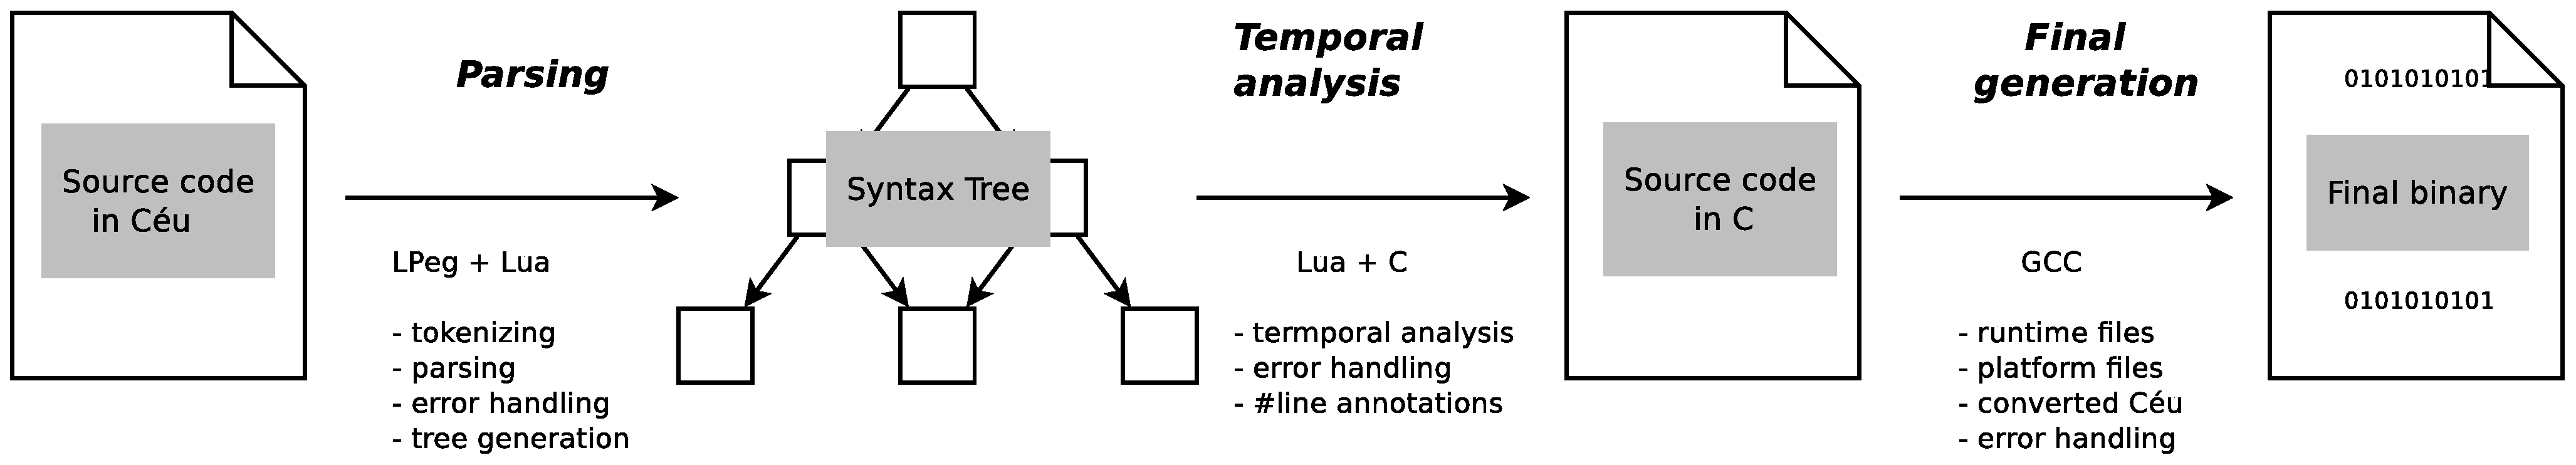
\includegraphics[scale=0.20]{impl}
\caption{ Compilation process: from the source code in \CEU to the final 
binary.
\label{fig.impl}
}
\end{figure}

\begin{comment}
The program below is used as our guiding example for this chapter:

\begin{lstlisting}[numbers=left,xleftmargin=2em]
input int A, B, C;
var int ret;
loop do
   par/or do
      do                            // 1st trail
          var int a = await A;
          ret = ret + a;
      end
      do
          var int b = await B;
          ret = ret + b;
      end
      break;
   with
      par/and do                    // 2nd trail
         finalize with
            ret = ret + 10;
         end
         await C;
      with
         await A;
      end
   end
end
...                                 // code after the loop
\end{lstlisting}
\end{comment}

\begin{description}

\item[Parsing]

The parser of \CEU is written in \emph{LPeg}~\cite{lua.lpeg}, a pattern 
matching library that also recognize grammars, making it possible to write the 
tokenizer and grammar with the same tool.
%
The source code is then converted to an \emph{abstract syntax tree (AST)} to be 
used in further phases.
%
This phase may be aborted due to syntax errors in the \CEU source file.

\item[Temporal Analysis]

This phase detects inconsistencies in \CEU programs, such as unbounded loops, 
suspicious accesses to shared memory, and also ``classical'' semantic analysis, 
such as building a symbol table for checking variable declarations.
%
This phase outputs code in \C, given the way \CEU is tied to \C by design.
%
Some type checking is delayed to the last phase to take advantage of 
\code{gcc}'s error handling.
Therefore, we annotate the \C output file with \code{\#line} pragmas matching 
the original file in \CEU.

\item[Code Generation]

The final phase packs the generated \C file with the \CEU runtime and 
platform-dependent functionality, compiling them with \emph{gcc} and generating 
the final binary.
%
The \CEU runtime comprehends the scheduler, timer management, and the external 
\C API.
%
The platform files include libraries for I/O and bindings to invoke the \CEU 
scheduler on external events.

\end{description}

%In the sections that follow, we discuss the most sensible parts of the 
%\emph{code generation} phase.
%compiler considering our design, such as the temporal analysis, runtime 
%scheduler, and the external API.

\subsection{Temporal Analysis for Shared-Memory Concurrency}

The compile-time \emph{temporal analysis} phase detects inconsistencies in \CEU 
programs.
Here, we focus on the algorithm that detects suspicious access to shared 
variables, as discussed in Section~\ref{sec.ceu.det}.

For each node representing a statement in the program AST, we keep the set of 
events $I$ (for \emph{incoming}) that can lead to the execution of the node, 
and also the set of events $O$ (for \emph{outgoing}) that can terminate the 
node.

A node inherits the set $I$ from its direct parent and calculates $O$ according 
to its type:
%
\begin{itemize}
%
\item Nodes that represent expressions, assignments, \C calls, and declarations 
simply reproduce $O=I$, as they do not await;
%
\item An \code{await e} statement has $O=\{e\}$.
%
\item A \code{break} statement has $O=\{\}$ as it escapes the innermost 
\code{loop} and never terminates, i.e., never proceeds to the statement 
immediately following it (see also \code{loop} below);
%
\item A \emph{sequence node (;)} modifies each of its children to have 
$I_n=O_{n-1}$.
The first child inherits $I$ from its parent node, and the set $O$ for the 
sequence node is copied from its last child, i.e., $O=O_n$.
%
\item A \code{loop} node includes its body's $O$ on its own $I$ ($I=I \cup 
O_{body}$), as the loop is also reached from its own body.
The union of all \code{break} statements' $O$ forms the set $O$ for a 
\code{loop}.
%
\item An \code{if} node has $O=O_{true} \cup O_{false}$.
%
\item A parallel composition may terminate from any of its branches, hence $O = 
O_1 \cup ... \cup O_n$.
\end{itemize}

With all sets calculated, we take all pairs of nodes that perform side effects 
and are in parallel branches, comparing their sets $I$ for intersections.
For each pair, if the intersection is not the empty set, we mark both nodes as 
suspicious.

The example in the left of Figure~\ref{lst.impl.ast} has a corresponding $AST$, 
in the right of the figure, with the sets $I$ and $O$ for each node.
The event $.$ (dot) represents the ``boot'' reaction.
The assignments to \code{y} in parallel (lines 5,8 in the code) have an empty 
intersection of $I$ (lines 6,9 in the AST), hence, they do not conflict.
Note that although the accesses in lines 5,11 in the code (lines 6,11 in the 
AST) do have an intersection, they are not in parallel and are also safe.

\begin{figure}
\begin{minipage}[t]{0.48\linewidth}
\begin{lstlisting}[numbers=left,xleftmargin=2.5em]
input void A, B;
var int y;
par/or do
  await A;
  y = 1;
with
  await B;
  y = 2;
end
await A;
y = 3;
\end{lstlisting}
\end{minipage}
%
%
\begin{minipage}[t]{0.48\linewidth}
\begin{lstlisting}[numbers=left,xleftmargin=2.5em]
Stmts I={.} O={A}
    Dcl_y I={.} O={.}
    ParOr I={.} O={A,B}
        Stmts I={.} O={A}
            Await_A I={.} O={A}
            Set_y I={A} O={A}
        Stmts I={.} O={B}
            Await_B I={.} O={B}
            Set_y I={B} O={B}
    Await_A I={A,B} O={A}
    Set_y I={A} O={A}
\end{lstlisting}
\end{minipage}
%
%\rule{14cm}{0.37pt}
\caption{ A program with a corresponding AST describing the sets $I$ and $O$.
%{\small %\textmd{
The program is safe because accesses to \code{y} in parallel have no 
intersections for $I$.
%}%}
\label{lst.impl.ast}
}
\end{figure}

\begin{comment}
It is also responsible for setting the priorities for trails (see further) and 
determining the sizes of the queues that are used during runtime.

The program AST is first converted into a graph that represents the execution 
flow.
Figure~\ref{fig:nfa} shows the corresponding graph for our example.

\begin{figure}
\centering
\includegraphics[scale=0.40]{nfa.png}
\caption{ Flow graph for our guiding example
\label{fig:nfa}
}
\end{figure}

By default, all nodes in a flow graph have priority $0$ (highest).
However, as the figure shows, nodes that represent the termination of 
\emph{par/ors} and loops have lower priorities (the outer, the lower).
The priority scheme is needed to avoid glitches during runtime, and is 
equivalent to traversing a dependency graph in topological order, as employed 
in functional reactive programming implementations.~\cite{frtime.embedding}

The flow graph is then converted to a DFA, as exemplified in 
Section~\ref{sec:ceu:det}.

From its starting node, the flow graph is traversed until reaching await 
nodes---every visited node is inserted into a new DFA state.
Then, every set of awaiting nodes for a given external event starts another DFA 
state.
\end{comment}

\subsection{Memory Layout}
\label{sec:impl:memory}

\CEU favors a fine-grained use of trails, being common the use of trails that 
await a single event.
For this reason, \CEU{} does not allocate per-trail stacks; instead, all data 
resides in fixed memory slots---this is true for the program variables as well 
as for temporary values and runtime flags.
%For instance, the first trail in the guiding example requires temporary slots 
%to hold the locals \code{a} and \code{b}, while the second trail must keep 
%flags to remember which sides of the \code{par/and} have already terminated.
%
Memory for trails in parallel must coexist, while statements in sequence can 
reuse it.
%
Translating this idea to \C is straightforward~\cite{wsn.osm,wsn.ocram}: memory 
for blocks in sequence are packed in a \code{struct}, while blocks in parallel, 
in a \code{union}.
%In the example, the code following the loop (identified as \code{...}) reuses 
%all memory from the loop.
%
\CEU reserves a single static block of memory to hold all memory slots, whose 
size is the maximum the program uses at a given time.
A given position in the memory may hold different data (with variable sizes) 
during runtime.
%
As an example, Figure~\ref{lst.impl.mem} shows a program with corresponding 
memory layout.
%
Each variable is assigned a unique $id$ (e.g. \code{a\_1}) so that variables 
with the same name can be distinguished.
%
The \code{do-end} blocks in sequence are packed in a \code{union}, given that 
their variables cannot be in scope at the same time, e.g., \code{MEM.a\_1} and 
\code{MEM.b\_2} can safely share the same memory slot.
%
The example also illustrates the presence of runtime flags related to the 
parallel composition, which also reside in reusable slots in the static memory.

\begin{figure}
\begin{minipage}[t]{0.48\linewidth}
\begin{lstlisting}
input int A, B, C;
do
    var int a = await A;
end
do
    var int b = await B;
end
par/and do
    await B;
with
    await C;
end
\end{lstlisting}
\end{minipage}
%
\begin{minipage}[t]{0.48\linewidth}
\begin{lstlisting}
union {             // sequence
    int a_1;        //   do_1
    int b_2;        //   do_2
    struct {        //   par/and
        int _and_3: 1;
        int _and_4: 1;
    };
} MEM ;
\end{lstlisting}
\end{minipage}
%\rule{14cm}{0.37pt}
\caption{
A program with blocks in sequence and in parallel, with corresponding memory 
layout that the compiler generates.
{\small %\textmd{
}%}
\label{lst.impl.mem}
}
\end{figure}

\subsection{Trail Allocation}
\label{sec:impl:gates}

Each line of execution in \CEU needs to carry associated data, such as which 
event it is awaiting and which code to execute when it awakes.
%
The compiler statically infers the maximum number of trails a program can have 
at the same time and creates a static vector to hold the runtime information 
about them.
%
Like normal variables, trails that cannot be active at the same time can share 
slots in the static memory vector.

At any given moment, a trail can be awaiting in one of the following states: 
\code{INACTIVE}, \code{STACKED}, \code{FIN}, or in any of the events defined in 
the program:

\begin{lstlisting}
enum {
    INACTIVE = 0,
    STACKED,
    FIN,
    EVT_A,      // input void A;
    EVT_e,      // event int e;
    <...>       // other events
}
\end{lstlisting}

All terminated or not-yet-started trails stay in the \code{INACTIVE} state and 
are ignored by the scheduler.
%
A \code{STACKED} trail holds an associated stack level and is delayed until the 
scheduler runtime reaches that level again.
%
A \code{FIN} trail represents a hanged finalization block which is only 
scheduled when its corresponding block goes out of scope.
%
A trail waiting for an event stays in the state of the corresponding event, 
also holding the minimum sequence number (\emph{seqno}) in which it can awake.
%
In concrete terms, a trail is represented by the following \code{struct}:

\begin{lstlisting}
struct trail_t {
    state_t evt;
    label_t lbl;
    union {
        unsigned char seqno;
        stack_t       stk;
    };
};
\end{lstlisting}

The field \code{evt} holds the state of the trail (or the event it is 
awaiting); the field \code{lbl} holds the entry point in the code to execute 
when the trail is scheduled; the third field depends on the \code{evt} field 
and may hold the \code{seqno} for an event, or the stack level \code{stk} for a
\code{STACKED} state.

The size of \code{state\_t} depends on the number of events in the application;
for an application with less than 253 events (plus the 3 states), one byte is 
enough.
%
The size of \code{label\_t} depends primarily on the number of \code{await} 
statements in the application---each \code{await} splits the code in two 
segments and requires a unique entry point in the code for its continuation.
Additionally, split \& join points for parallel compositions, \code{emit} 
continuations, and finalization blocks also require labels.
%
The \code{seqno} could eventually overflow during execution (i.e., every 256 
reactions).
However, given that the scheduler traverses all trails on every reaction, it 
can adjust them to properly handle overflows (actually, 2 bits to hold the 
\code{seqno} is already enough).
%
The size of \code{stack\_t} depends on the maximum depth of nested emissions 
and is bounded to the maximum number of trails.
In the worst case, a trail emits an event that awakes another trail, which 
emits an event that awakes another trail, and so on.
The last trail cannot awake any trail, because they are all hanged in the 
\code{STACKED} state.

In the context of embedded systems, the size of \code{trail\_t} is typically 
only 3 bytes (1 byte for each field), imposing a negligible memory overhead 
even for trails that only await a single event and terminate.
%
For instance, the \emph{CTP} collection protocol ported to \CEU reaches eight 
simultaneous lines of execution with an overhead of 2\% in comparison to the 
original version in \emph{nesC}~\cite{wsn.nesc} (a dialect of \C for 
event-driven programming)~\cite{ceu.sensys13}.

\subsection{Code Generation and Scheduling}

\begin{figure}
\begin{minipage}[t]{0.31\linewidth}
\begin{lstlisting}
input void A;
event void e;
// TRAIL 0 - lbl Main
par/and do
  // TRAIL 0 - lbl Main
  await e;
  // TRAIL 0 - lbl Awake_e
  // TRAIL 0 - lbl And_chk
with
  // TRAIL 1 - lbl And_sub_2
  await A;
  // TRAIL 1 - lbl Awake_A_1
  emit e;
  // TRAIL 1 - lbl Emit_cont
  // TRAIL 1 - lbl And_chk
end
// TRAIL 0 - lbl And_out
await A;
// TRAIL 0 - lbl Awake_A_2





.
\end{lstlisting}
\end{minipage}
%
\begin{minipage}[t]{0.31\linewidth}
\begin{lstlisting}[numbers=left,xleftmargin=2.5em]
enum {
  Main = 1,  // ln 3
  Awake_e,   // ln 7
  And_chk,   // ln 8,15
  And_sub_2, // ln 10
  Awake_A_1, // ln 12
  Emit_cont, // ln 14
  And_out,   // ln 17
  Awake_A_2  // ln 19
};

trail_t TRLS[2] = {
  { STACKED,  Main, 0 };
  { INACTIVE, 0,    0 };
};









.
\end{lstlisting}
\end{minipage}
%
\begin{minipage}[t]{0.37\linewidth}
\begin{lstlisting}[numbers=left,xleftmargin=2.5em]
void dispatch (trail_t* t) {
  switch (t->lbl) {
    case Main:
      // activate TRAIL 1
      TRLS[1].evt = STACKED;
      TRLS[1].lbl = And_sub_2;
      TRLS[1].stk = cur_stack;
  
      // code in the 1st trail
      // await e;
      TRLS[0].evt = EVT_e;
      TRLS[0].lbl = Awake_e;
      TRLS[0].seq = cur_seqno;
      break;
  
    case And_sub_2:
      // await A;
      TRLS[1].evt = EVT_A;
      TRLS[1].lbl = Awake_A_1;
      TRLS[1].seq = cur_seqno;
      break;
  
    <...>  // other labels
  }
}
\end{lstlisting}
\end{minipage}
\caption{
%{\small %\textmd{
From left to right: static allocation of trails, entry-point labels, and 
dispatch function.
In the left, the comments identify the trail indexes inferred by the compiler.
In the middle, each trail segment has an associated numeric identifier 
generated by the compiler.
In the right, the dispatcher uses a \code{switch} to associate each segment 
identifier with the corresponding code to execute.
%}%}
\label{lst.impl.trails}
}
\end{figure}

In the final generated code in \C, each trail label representing an entry point 
becomes a \emph{switch case} with the associated code to execute.
%
Figure~\ref{lst.impl.trails} illustrates the generation process.
For the program in the left of the figure, the compiler extracts the entry 
points and associated trails, e.g., the label \code{Awake\_e} will execute on 
\code{TRAIL-0} (line 7).
%
For each statement that pauses (\code{emit} and \code{await}), resumes 
(\code{par/and}, \code{par/or}, and \code{finalize}), or aborts (\code{par/or} 
and \code{break}), the compiler splits the trail into segments with associated 
entry points.
%
The entry points translate to an \code{enum} in the generated code (lines 
1--10, in the middle of the figure).
The state of trails translate to a vector of type \code{trail\_t} with the 
maximum number of simultaneous trails (lines 12--15).
On initialization, \code{TRAIL-0} is set to execute the \code{Main} entry point 
(line 13), while all others are set to \code{INACTIVE} (in the example, only 
one, in line 14).

The scheduler executes in two passes:
%
In the \emph{broadcast} pass, the scheduler sets all trails that are waiting 
for the current event to \code{STACKED} in the current stack level.
%
In the \emph{dispatch} pass, the scheduler executes each trail that is 
\code{STACKED} to run in the current level, setting it immediately to 
\code{INACTIVE}.

During the dispatch pass, if a trail executes and emits an internal event, the 
scheduler increments the stack level and re-executes the two passes.
After all trails are properly dispatched, the scheduler decrements the stack 
level and resumes the previous execution.
For the first reaction chain, the scheduler starts from the \emph{dispatch} 
pass, given that the \code{Main} label is the only one that can be active at 
the stack level 0 (line 13, in the middle of Figure~\ref{lst.impl.trails}).

The code the right of the Figure~\ref{lst.impl.trails} dispatches a trail
according to the current label to execute.
%
For the first reaction, it executes the \code{Main} label in \code{TRAIL-0}.
%
When the \code{Main} label reaches the \code{par/and}, it stacks \code{TRAIL-1} 
(lines 4--7) and proceeds to the code in \code{TRAIL-0} (lines 9--14), 
respecting the deterministic execution order.
%
The code sets the running \code{TRAIL-0} to await \code{EVT\_e} on label 
\code{Awake\_e}, and then halts with a \code{break}.
%
The next iteration of \code{dispatch} takes \code{TRAIL-1} and executes its 
registered label \code{And\_sub\_2} (lines 16--21), which sets \code{TRAIL-1} 
to await \code{EVT\_A} and also halts.

Regarding abortion and finalization, when a \code{par/or} terminates, the 
scheduler makes a \emph{broadcast} pass for the \code{FIN} event, but limited 
to the range of trails covered by the terminating \code{par/or}.
Trails that do not match the \code{FIN} are set to \code{INACTIVE}, as they 
have to be aborted.
Given that trails in parallel are allocated in subsequent slots in the static 
vector \code{TRLS}, this pass only aborts the desirable trails.
The subsequent \emph{dispatch} pass executes the finalization code.
%Given that finalization blocks cannot contain \code{await} statements, the 
%whole process is guaranteed to terminate in bounded time.
Escaping a \code{loop} that contains parallel compositions also triggers the 
same abortion process.

\subsection{The External \C API}

As a reactive language, the execution of a program in \CEU is guided entirely 
by the occurrence of external events.
From the implementation perspective, there are three external sources of input 
into programs, which are all exposed as functions in a \C API:

\begin{description}
\item[{\textbf\code{ceu\_go\_init()}}:] initializes the program (e.g. trails) 
and executes the ``boot'' reaction (i.e., the \code{Main} label).

\item[{\textbf\code{ceu\_go\_event(id,param)}}:] executes the reaction for the 
received event id and associated parameter.

\item[{\textbf\code{ceu\_go\_wclock(us)}}:] increments the current time in 
microseconds and runs a reaction if any timer expires.

%\item[{\textbf\code{ceu\_go\_async}}:] executes a single loop iteration for 
%the next \code{async}, switching among them in a \emph{round robin} policy.
\end{description}

Given the semantics of \CEU, the functions are guaranteed to take a bounded 
time to execute.
They also return a status code that says if the \CEU{} program has terminated 
after the reactions.
Further calls to the API have no effect on terminated programs.

\begin{comment}
Note that \CEU{} code running from a call to \code{ceu\_go\_async} may emit an 
input event or the passage of time.
In this case, the \C implementation makes a tail call to the corresponding 
handler (i.e.  \code{ceu\_go\_event} or \code{ceu\_go\_time}), as synchronous 
code has higher priority.

The API reflects the \emph{global asynchronous} part of \CEU{}, as discussed in 
Section~\ref{sec:ceu:gals}.
A simple and opaque API hides local state from the environment, suggesting that 
the execution varies entirely according to the sequence (and parameters) of API 
calls.
\end{comment}

The bindings for the specific platforms are responsible for calling the 
functions in the API in the order that better suit their requirements.
As an example, it is possible to set different priorities for events that occur 
concurrently (i.e. while a reaction chain is running).
However, a binding must never interleave or run multiple functions in parallel.
This would break the \CEU sequential/discrete semantics of time.
%, as discussed in Section~\ref{sec:ceu}.

\begin{figure}
\begin{lstlisting}[numbers=left,xleftmargin=2em]
implementation
{
    #include "ceu.h"
    #include "ceu.c"

    event void Boot.booted () {
        ceu_sys_init();
#ifdef CEU_WCLOCKS
        call Timer.startPeriodic(10);
#endif
    }
    
#ifdef CEU_WCLOCKS
    event void Timer.fired () {
        ceu_sys_wclock(10000);
    }
#endif

#ifdef EVT_PHOTO_READDONE
    event void Photo.readDone (uint16_t val) {
        ceu_sys_go(EVT_PHOTO_READDONE, &val);
    }
#endif

#ifdef EVT_RADIO_SENDDONE
    event void RadioSend.sendDone (message_t* msg) {
        ceu_sys_go(EVT_RADIO_SENDDONE, &msg);
    }
#endif

#ifdef EVT_RADIO_RECEIVE
    event message_t* RadioReceive.receive (message_t* msg) {
        ceu_sys_go(EVT_RADIO_RECEIVE, &msg);
        return msg;
    }
#endif

    <...>   // other events
}
\end{lstlisting}
%\rule{14cm}{0.37pt}
\caption{
%{\small %\textmd{
The \emph{TinyOS} binding for \CEU.
%}%}
\label{lst.impl.tinyos}
}
\end{figure}

As an example, Figure~\ref{lst.impl.tinyos} shows our binding for 
\emph{TinyOS}~\cite{wsn.tos}, which maps callbacks to input events in \CEU.
%
The file \code{ceu.h} (included in line 3) contains all definitions for the 
compiled \CEU program, which are further queried through \code{\#ifdef}'s.
The file \code{ceu.c} (included in line 4) contains the main loop of \CEU 
pointing to the labels defined in the program.
The callback \code{Boot.booted} (lines 6--11) is called by TinyOS on startup, 
so we initialize \CEU inside it (line 7).
If the \CEU program uses timers, we also start a periodic timer (lines 8--10) 
that triggers callback \code{Timer.fired} (lines 13--17) every 10 milliseconds 
and advances the wall-clock time of \CEU (line 15)%
\footnote{We also offer a mechanism to start the underlying timer on demand to
avoid the ``battery unfriendly'' 10ms polling.}.
The remaining lines map pre-defined TinyOS events that can be used in \CEU 
programs, such as the light sensor (lines 19--23) and the radio transceiver 
(lines 25--36).

\subsection{The Terra Virtual Machine}
\label{sec.terra}

Terra is a system for programming wireless sensor network applications that 
uses \CEU as its scripting language~\cite{ceu.terra}.
%
Figure \ref{fig.terra} shows the three basic elements of Terra:
\CEU as the scripting language,
a set of customized pre-built components,
and the embedded virtual-machine engine which can disseminate and install 
bytecode images dynamically.
%
This approach aims to combine the flexibility of remotely uploading code with 
the expressiveness and safety guarantees of \CEU.

\begin{figure}[!htb]
 \centering
 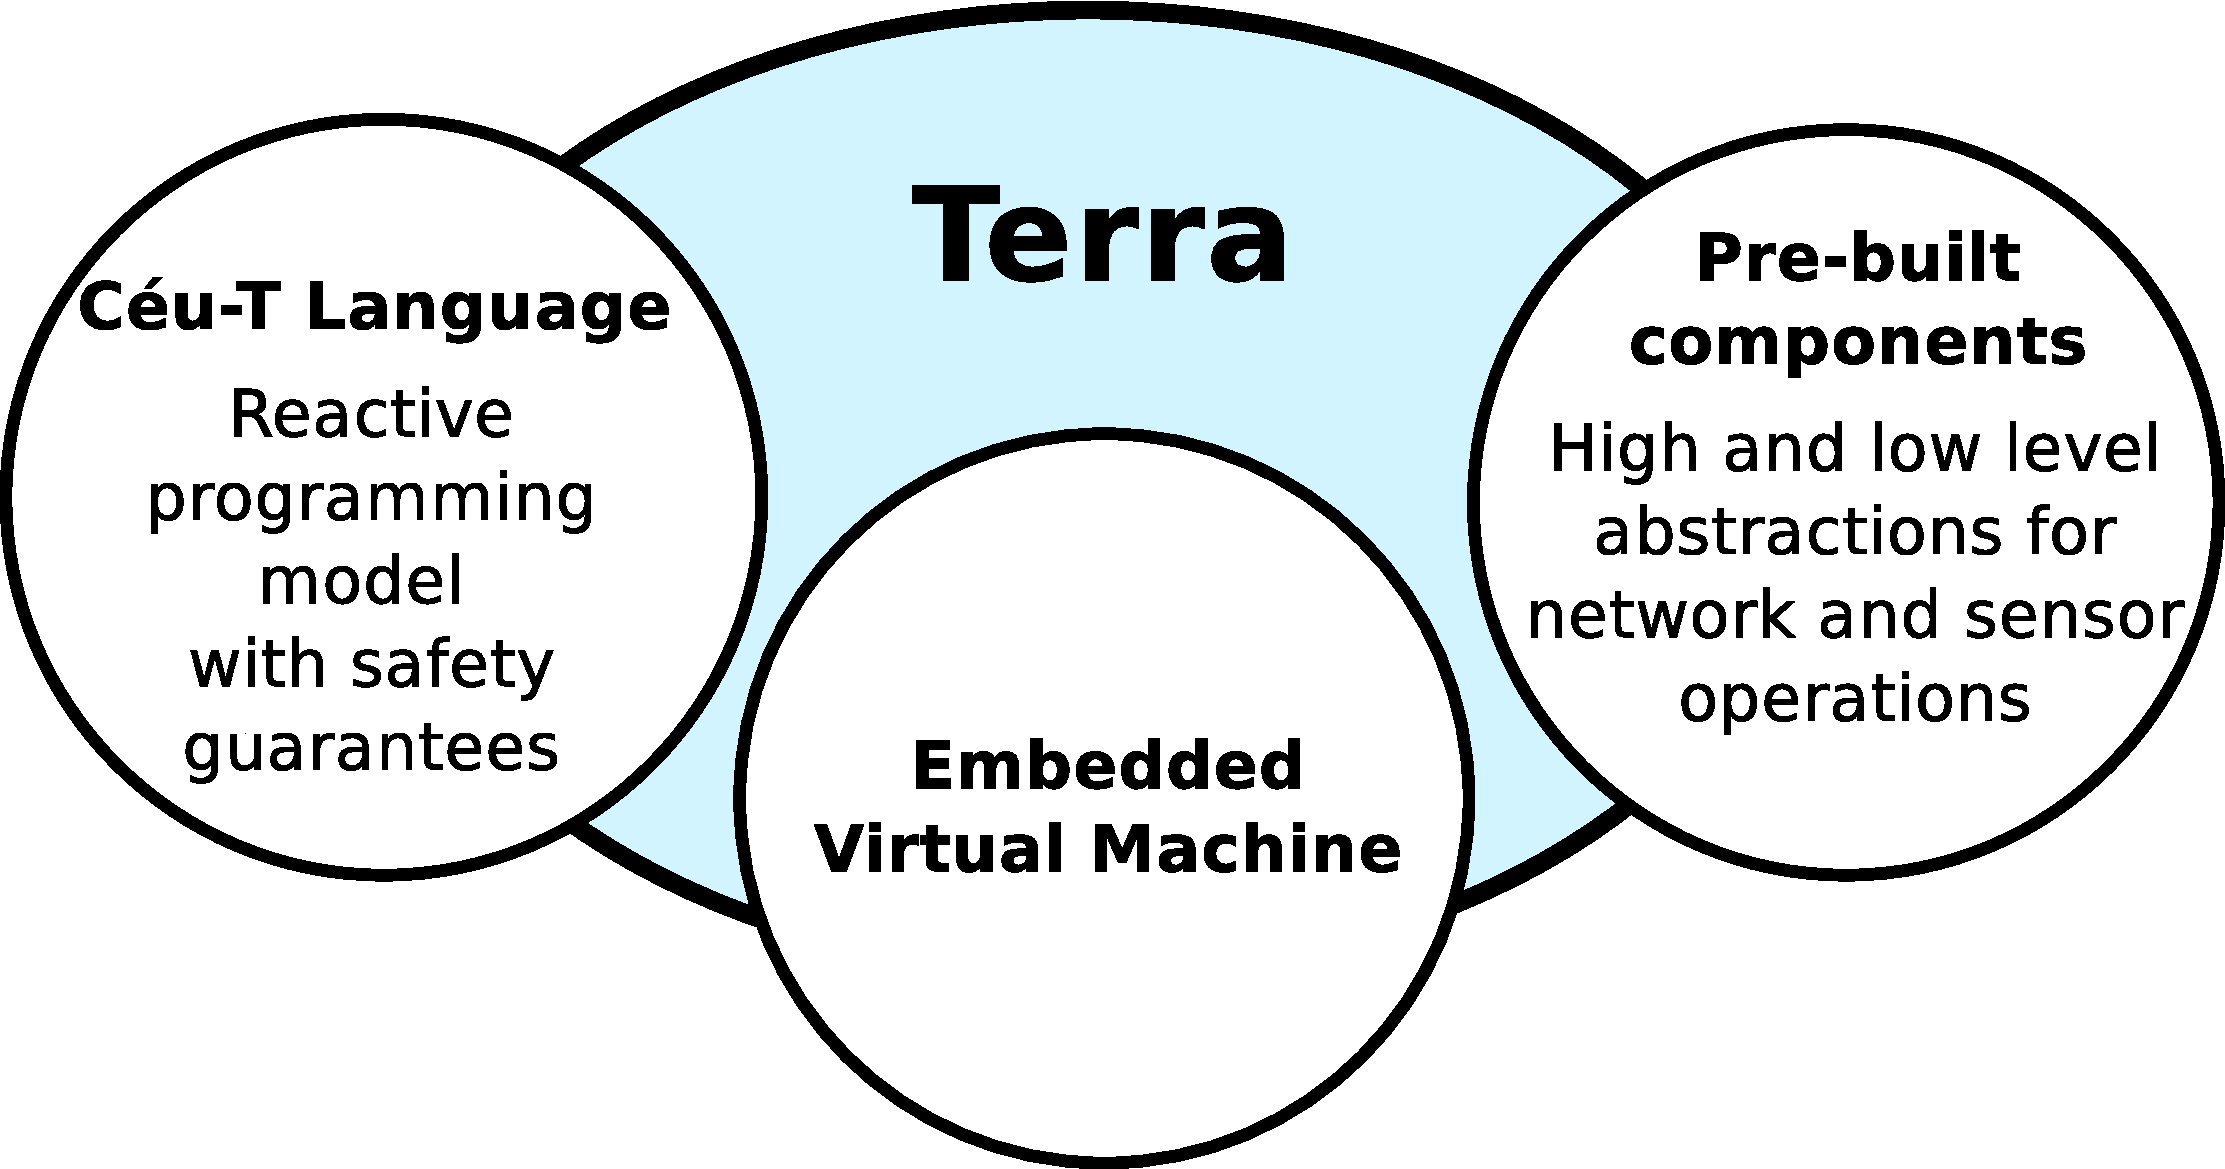
\includegraphics[width=0.5\columnwidth]{terra}
\caption{Terra programming system basic elements.}
 \label{fig.terra}
\end{figure}

In Terra, \CEU scripts cannot execute arbitrary \C code, instead, they rely on 
pre-built components that can be customized for different application domains.
%
Considering the domain of sensor networks, Terra already provides components 
organized in four areas: radio communication, group management, data 
aggregation, and local operations (e.g., access to sensors and actuators).
%
When creating an instance of the \VM, the programmer can choose whether or not 
to include each component, setting different abstraction boundaries for 
scripts.
%
The generated \VM has to be preloaded into the embedded devices before they are 
physically distributed.

The communication between scripts in \CEU and the components in the \VM is 
mostly through events:
scripts \code{emit} requests through \code{output} events and \code{await} 
answers through \code{input} events.
%
Terra also provides system calls for initialization and configuration of 
components.
%
TODO: explicar Figura 21.
\begin{comment}
Figure~\ref{lst.terra.defs} illustrates a program interface declaration in \CEU
(in the left), and associated binding code in \C

 with respective binding customization scenario.
This customization sample uses a small data structure, two output events, one input event, and two functions.
The left listing is the definition file to be included into the \CEU script program and the right listing is the
definition file to be included into the VM custom module implementation.
\end{comment}

\begin{figure}
\begin{minipage}[t]{0.46\linewidth}
\begin{lstlisting}[morekeywords={ubyte,ushort,output,function,regtype}]
// Message definition
regtype sensorMsg with
    var ubyte  id;
    var ushort value;
end

// Output events definition
output void REQ_TEMP void          1;
output void SEND_SENSOR sensorMsg  2;

// Input events definition
input void TEMP void               1;

// functions definitions
function ubyte getNodeId()         1;
function ubyte queuePut(sensorMsg) 2;
.
\end{lstlisting}
\end{minipage}
%
\begin{minipage}[t]{0.51\linewidth}
\begin{lstlisting}[numbers=left,xleftmargin=2.5em,
morekeywords={nx_struct,nx_uint8_t,nx_uint16_t,uint8_t,uint32_t}]

typedef nx_struct sensorMsg{
  nx_uint8_t  id;
  nx_uint16_t value;
} sensorMsg_t;

enum {
  O_REQ_TEMP    = 1;
  O_SEND_SENSOR = 2;

 
  I_TEMP        = 1;

 
  F_GETNODEID   = 1;
  F_QUEUEPUT    = 2;
};

\end{lstlisting}
\end{minipage}
\caption{
%{\small %\textmd{
Terra control block sample and the equivalent definition for VM implementation.
%}%}
\label{lst.terra.defs}
}
\end{figure}

TODO: dizer o que eh manual/automatico nos lsts de ceu

TODO-VM: exemplo de implementacao/uso de um componente
- Terra: binding em nesC
- Ceu: header de configuracao
- (analogo a Figura 19)

Considering the compilation process illustrated in Figure~\ref{fig.impl} for 
the \C back end, the main difference resides in the \emph{Code Generation} 
phase, which here outputs assembly instructions for the Terra \VM, instead of 
\C.

TODO-VM: falar um pouco do assembly/bytecode, quais as decisoes envolvidas
- (analogo a Figura 18)

\begin{comment}
%-------------------------------------------------
Figure~\ref{lst.impl.custom} presents a partial implementation for the elements 
introduced in the Figure~\ref{lst.impl.defs}.
The two first functions are called from the VM decoder, the fist function \code{procOutevt()} dispatch any defined output events
and the function \code{callFunction()} dispatch any defined customized functions.
Lines 17--22 shows an example of a custom function that returns a value via stack.
Lines 24--27 has a example of an external event call.
Lines 29--34 presents an example how a input event is queued to the VM engine.
\end{comment}
 
%-----------------------------------------------------
% Equivalent to the fig. 19

\begin{figure}
\begin{minipage}[t]{0.81\linewidth}
\begin{lstlisting}[numbers=left,xleftmargin=2.5em,
morekeywords={uint8_t,uint16_t,uint32_t,error_t,command}]
// Output event dispatcher
command void VM.procOutEvt(uint8_t id, uint32_t value){
  switch (id){
    case O_REQ_TEMP    : proc_req_temp(id,value);    break;
    case O_SEND_SENSOR : proc_send_sensor(id,value); break;
  }
}

// Function dispatcher
command void VM.callFunction(uint8_t id){
  switch (id){
    case F_GETNODEID : func_getNodeId(id); break;
    case F_QUEUEPUT  : func_queuePut(id);  break;
  }
}

// Pushing a value to the stack
void  func_getNodeId(uint16_t id){
  uint16_t stat;
  stat = TOS_NODE_ID;
  signal VM.push(stat);
}

// Calling a output event
void  proc_req_temp(uint16_t id, uint32_t value){
  call S_TEMP.read();
}

// Queueing an input event + value
uint16_t lastTemp;
event void S_TEMP.readDone(error_t result, uint16_t val)
  lastTemp = val;
  signal VM.queueEvt(I_TEMP, 0, &lastTemp);
}

\end{lstlisting}
\end{minipage}

\caption{
%{\small %\textmd{
VM Customization -- input/output events and functions.
%}%}
\label{lst.impl.custom}
}
\end{figure}

%------------------------------------------------------

\begin{comment}
Instead of generating code in C, Terra generates the vmt assembly code using 
the original Céu labels for trails entry points.
In the final phase for code generation, Terra compiler generates the vmt 
bytecode file using the program address in place of Céu labels.
The use of address allows the Céu scheduler to execute directly a trail without 
a index table to replace the switch-case.
Related to memory layout and trail allocation, Terra uses the same data 
organization approach for all Céu controls and variables.
All Céu data and control structures for a specific program are determined at 
compile time.
Terra arranges all these structures in the beginning of virtual machine memory 
space.
The original Céu run time control functions are maintained with a small 
modification where accesses to control structures have an off-set relative to 
the begin of the virtual machine memory space.
\end{comment}

\section{Related Work}
\label{sec.related}

\emph{(As subsecoes serao retiradas do texto ao final...)}

\subsection{Semantics}

\CEU has a strong influence from Esterel~\cite{esterel.ieee91} and embraces the 
disciplined synchronous-reactive model and support for lexical composition of 
lines of execution.
%
However, there are fundamental semantic differences that prevents the design of 
\CEU as pure extensions to Esterel (i.e., on top of its formal semantics).
%
In particular, Esterel has a notion of time similar to that of digital circuits 
in which multiple signals can be active at a clock tick.
In fact, Esterel is also used in hardware design.
%
In \CEU, instead of clock ticks, the occurrence of a single external event that 
defines a time unit.
%
\CEU also distinguishes external events from stack-based internal events, which 
provide a limited form of coroutines supporting reactive statements (e.g., 
\code{await} and \code{par/or}).

The event-driven approach of \CEU is well known~\cite{sync_async.whynotthreads} 
and popular in many software communities, such as client and server-side web 
frameworks (e.g., \emph{jQuery}~\cite{js.jquery} and 
\emph{Node.js}~\cite{js.node}), GUI toolkits (e.g., \emph{Tcl/Tk}~\cite{tcl.tk} 
and \emph{Java Swing}~\cite{java.swing}), and Games~\cite{gamepatterns}.
%
Like \CEU, event-driven programming is essentially synchronous, i.e., events go 
through a queue and are dispatched sequentially and atomically to prevent race 
conditions.
%
We believe that for software design, this approach is more familiar to 
programmers and simplifies the reasoning about concurrency.
For instance, the uniqueness of external events in \CEU is a prerequisite for 
the temporal analysis that enables safe shared-memory concurrency.

A number of synchronous languages have been designed to interoperate with C, 
such as \emph{Reactive C}~\cite{rp.rc}, Protothreads~\cite{wsn.protothreads}, 
\emph{PRET-C}~\cite{rp.pretc} and \emph{SC}~\cite{rp.synchc}.
%
They offer Esterel-like parallel compositions with communication via shared 
variables, relying on deterministic scheduling to preserve determinism.
%
However, it is the responsibility of the programmer to specify the execution 
order for threads, based on either explicit priorities, or source code lexical 
order (like \CEU).
%
These languages have a tick-based notion of time similar to Esterel, which 
prevents the event-based temporal analysis of \CEU.

\emph{URBI}~\cite{rp.urbi} is a reactive scripting language with a rich set of 
control constructs for time management, event-driven communication, and 
concurrency.
Concurrency is based on stackful coroutines, diverging from our goals regarding 
resource efficiency and static bounds for memory and execution time.

TODO-VM

\begin{comment}
More recently, Wireless Sensor Networks (WSNs) emerged as an active research 
area for highly constrained embedded concurrency, resulting in the development 
of many synchronous languages~\cite{wsn.protothreads,wsn.sol,wsn.osm}.
%
offer lightweight cooperative multi-threading for embedded systems.
Its stackless implementation reduces memory consumption but precludes support 
for local variables.
\CEU also avoids the use of stacks for trails, but preserves support for locals 
by calculating the required memory at compile time.
%
SOL~\cite{wsn.sol} and OSM~\cite{wsn.osm} provide parallel state machines for 
WSNs, offering a formal and mature model for programming embedded systems.
However, the main contributions of \CEU, stacked execution for internal 
events and safe support for shared-memory concurrency, do not directly adapt to 
the state-machine formalism.

In common among the referred works is the agreement in providing low-level 
access (e.g., systems calls and shared-memory) and lock-free concurrency that 
precludes race conditions on programs.
However, they do not specify an execution order for tasks reacting to the same 
external stimulus~\cite{esterel.primer,wsn.protothreads,wsn.osm}.
This way, if two tasks access the same resource concurrently, even if the 
accesses are race free, the final outcome is nondeterministic.
As discussed in Section~\ref{sec.safety.det}, \CEU refuses programs with such 
behavior.

On the opposite side of the spectrum of concurrency models, asynchronous 
languages for embedded systems~\cite{wsn.mantisos,arduino.occam}
assume time independence among processes and are more appropriate for 
applications with a low synchronization rate or for those involving
algorithmic-intensive problems.
\end{comment}

\subsection{Implementation}

Esterel has different compilation back ends that synthesizes to software and 
also to hardware circuits~\cite{esterel.emperor,esterel.tutorial}.
Among the software-based approaches, \emph{SAXO--RT}~\cite{esterel.saxort} is 
the closest to our implementation with respect to trail allocation and 
scheduling:
the compiler slices programs into ``control points'' (analogous to our ``entry 
points'') and rearranges them into a directed acyclic graph respecting the 
constructive semantics of Esterel.
Then, it flattens the graph into sequential code in \C suitable for static 
scheduling.

TODO-VM

\begin{comment}
- Kiel Esterel compiler

- We are not concerned with WCET:
Predictable system design is concerned with the challenge o
f building sys-
tems in such a way that requirements can be guaranteed from th
e design. This
means that an off-line analysis should demonstrate satisfa
ction of timing require-
ments, subject to assumptions made on operating conditions
foreseen for the sys-
tem [Stankovic and Ramamritham 1990]

http://embedded.cs.uni-saarland.de/publications/BuildingTimingPredictableEmbeddedSystems.pdf
survey of timeing-predictable embedded systems,
synchronous languages do some at the lang semantic level
\cite{pret.building}
\end{comment}

\section{Conclusion}
\label{sec.conclusion}

We presented the design, semantics, and implementation of \CEU, a synchronous 
reactive language based on Esterel targeting constrained embedded systems.

\CEU is a concurrency-safe language, employing a static analysis that encompass 
all control constructs and ensures that the high degree of concurrency in 
embedded systems does not pose safety threats to applications.
%
As a summary, the following safety properties hold for all programs that 
successfully compile in \CEU:
time and memory-bounded reactions to the environment (except for external 
system calls),
no race conditions in shared memory,
reliable abortion for activities handling resources,
and automatic synchronization for timers.
%
These properties are usually desirable in applications and are guaranteed as 
preconditions in \CEU by design.

\CEU is a resource-efficient language suitable for constrained embedded 
systems.
The reference implementation compiles to portable event-driven code in \C, with 
no special requirements for OS threads or per-trail data stacks.
The \VM implementation uses the same front end and imposes no extra 
restrictions, being equally suitable for constrained systems.

\CEU is a practical language with expressive control constructs, such as 
lexically scoped parallel compositions, convenient first-class timers, and a 
unique stack-based signaling mechanism.
%
Programs interoperate seamlessly with \C, and can take advantage of existing 
libraries, lowering the entry barrier for adoption.
%
\CEU has an open source implementation and bindings for \emph{TinyOS}, 
\emph{Arduino}, and the \emph{SDL} graphical library.%
\footnote{Website of \CEU: \url{http://www.ceu-lang.org/}}

For the past three years, we have been teaching \CEU for undergraduate and 
graduate students in research projects and two hands-on courses on 
\emph{distributed systems} and \emph{reactive programming}.
%, in which the studnets designing protocols, embedded systems, and graphical 
%applications.
%
Our experience shows that students take advantage of the sequential-imperative 
style of \CEU and can implement non-trivial concurrent applications in a few of 
weeks.

% Idexx

\begin{comment}
We are also extending and applying \CEU in more dynamic domains, such as GUIs 
and games~\cite{ceu.mod15}, by relaxing some restrictions in the language.
In particular, programs in these domains typically require unbounded memory and 
execution time, such as for dealing with dynamic collections.
We provide unsafe annotations to circumvent the rigid semantics of \CEU, 
requiring them to be explicit and trackable at the same time.
\end{comment}

% Bibliography
\bibliographystyle{ACM-Reference-Format-Journals}
\bibliography{my,other,terra}
                             % Sample .bib file with references that match those in
                             % the 'Specifications Document (V1.5)' as well containing
                             % 'legacy' bibs and bibs with 'alternate codings'.
                             % Gerry Murray - March 2012

% History dates
%\received{February 2007}{March 2009}{June 2009}

% Electronic Appendix
%\elecappendix

%\medskip

\end{document}
% End of v2-acmsmall-sample.tex (March 2012) - Gerry Murray, ACM
